\documentclass[review]{elsarticle}
 
\usepackage{lineno,hyperref}
\modulolinenumbers[5]

\journal{Journal of \LaTeX\ Templates}

%%%%%%%%%%%%%%%%%%%%%%%
%% Elsevier bibliography styles
%%%%%%%%%%%%%%%%%%%%%%%
%% To change the style, put a % in front of the second line of the current style and
%% remove the % from the second line of the style you would like to use.
%%%%%%%%%%%%%%%%%%%%%%%

%% Numbered
%\bibliographystyle{model1-num-names}

%% Numbered without titles
%\bibliographystyle{model1a-num-names}

%% Harvard
%\bibliographystyle{model2-names.bst}\biboptions{authoryear}

%% Vancouver numbered
%\usepackage{numcompress}\bibliographystyle{model3-num-names}

%% Vancouver name/year
\usepackage{numcompress}\bibliographystyle{model4-names}\biboptions{authoryear}

%% APA style
%\bibliographystyle{model5-names}\biboptions{authoryear}

%% AMA style
%\usepackage{numcompress}\bibliographystyle{model6-num-names}

%% `Elsevier LaTeX' style
%\bibliographystyle{elsarticle-num}
%%%%%%%%%%%%%%%%%%%%%%%
\usepackage{xeCJK}
\usepackage{bm}
\usepackage{amsmath}
\usepackage{amssymb}
\usepackage{amsthm}
\usepackage{graphicx}
\usepackage{color}
\usepackage{booktabs}

\DeclareMathOperator{\mytr}{tr}
\DeclareMathOperator{\mydiag}{diag}
\DeclareMathOperator{\myrank}{Rank}
\DeclareMathOperator{\myE}{E}
\DeclareMathOperator{\myVar}{Var}





\theoremstyle{plain}
\newtheorem{theorem}{\quad\quad Theorem}
\newtheorem{proposition}{\quad\quad Proposition}
\newtheorem{corollary}{\quad\quad Corollary}
\newtheorem{lemma}{\quad\quad Lemma}
\newtheorem{example}{Example}
\newtheorem{assumption}{\quad\quad Assumption}
\newtheorem{condition}{Condition}

\theoremstyle{definition}
\newtheorem{remark}{\quad\quad Remark}
\theoremstyle{remark}
\begin{document}

\begin{frontmatter}

\title{High-dimensional two-sample test under spiked covariance}

%% Group authors per affiliation:
    \author[mymainaddress]{Rui Wang}
    \author[mymainaddress,mysecondaryaddress]{Xingzhong Xu\corref{mycorrespondingauthor}}
\cortext[mycorrespondingauthor]{Corresponding author}
\ead{xuxz@bit.edu.cn}
    \address[mymainaddress]{School of Mathematics and Statistics, Beijing Institute of Technology, Beijing 
    100081,China}
    \address[mysecondaryaddress]{Beijing Key Laboratory on MCAACI, Beijing Institute of Technology, Beijing 100081,China}
%\fntext[myfootnote]{Since 1880.}

%% or include affiliations in footnotes:
%\author[mymainaddress,mysecondaryaddress]{Elsevier Inc}
%\ead[url]{www.elsevier.com}



\begin{abstract}
    This paper considers testing the means of two $p$-variate normal samples in high dimensional setting.  The covariance matrices are assumed to be spiked, which often arises in practice. 
    We propose a new test procedure through projection on the orthogonal complement of principal space.
    The asymptotic normality of the new test statistic is proved and the power function of the test is given.
    Theoretical and simulation results show that the new test outperforms existing methods substantially when the covariance matrices are spiked. Even when the covariance matrices are not spiked, the new test is acceptable.
\end{abstract}

\begin{keyword}
    high dimension, mean test, orthogonal complement of principal space, spiked covariance
\end{keyword}

\end{frontmatter}

%\linenumbers



\section{Introduction}

Suppose that $X_{k,1},\ldots,X_{k,n_k}$  are independent identically distributed (i.i.d.) as $N_p(\mu_k,\Sigma_k)$, where $\mu_k$ and $\Sigma_k$ are unknown, $k=1,2$. We consider the hypothesis testing problem:

\begin{equation}\label{problem}
    H_0:\mu_1=\mu_2\quad \textrm{vs.}\quad H_1:\mu_1\neq \mu_2.
\end{equation}
 In this paper, high dimensional setting is adopted, i.e., the dimension $p$ varies as $n$ increase, where $n=n_1+n_2$ is the total sample size.
Testing hypotheses~\eqref{problem} is important in many applications, including biology, finance and economics.
Quite often,  these data have strong correlations between variables.
When strong correlations exist, covariance matrices are often spiked in the sense that a few eigenvalues are distinctively larger than the others.
This paper is devoted to
testing hypotheses~\eqref{problem} in high dimensional setting with spiked covariance.


If $\Sigma_1=\Sigma_2=\Sigma$ is unknown, a classical test for hypotheses~\eqref{problem} is Hotelling's $T^2$ test.  Hotelling's test statistic is ${(\bar{X}_1-\bar{X}_2)}^T S^{-1}(\bar{X}_1-\bar{X}_2)$, where $S$ is the pooled sample covariance matrix. However, Hotelling's test is not defined when $p\geq n-1$.
Moreover,~\cite{Bai1996Efiect} showed that even if $p<n-1$, Hotelling's test suffers from low power when $p$ is comparable to $n$.
Perhaps, the main reason for low power of Hotelling's test is due to that $S$ is a poor estimator of $\Sigma$ when $p$ is large compared with $n$. See~\cite{Chen2010A} and the references therein.
In high dimensional setting,  
many test statistics in the literatures are based on an estimator of ${(\mu_1-\mu_2)}^T A(\mu_1-\mu_2)$ for a given positive definite matrix $A$. 
For example,~\cite{Bai1996Efiect} proposed a test based on
\begin{equation*}
    T_{BS}=\|\bar{X}_1-\bar{X}_2\|^2-(\frac{1}{n_1}+\frac{1}{n_2})\mathrm{tr}S,
\end{equation*}
which is an unbiased estimator of $\|\mu_1-\mu_2\|^2$.~\cite{Chen2010A} modified $T_{BS}$ by removing terms $\sum_{i=1}^{n_k}X_{ki}^T X_{ki}$, $k=1,2$ and proposed a test based on
\begin{equation*}
    \begin{aligned}
        T_{CQ}&=\frac{\sum_{i\neq j}^{n_1}X_{1i}^T X_{1j}}{n_1(n_1-1)}+\frac{\sum_{i\neq j}^{n_2}X_{2i}^T X_{2j}}{n_2(n_2-1)}-2\frac{\sum_{i=1}^{n_1}\sum_{j=1}^{n_2}X_{1i}^T X_{2j}}{n_1n_2}
        \\
            &=\|\bar{X}_1-\bar{X}_2\|^2-\frac{1}{n_1}\mathrm{tr}S_1-\frac{1}{n_2}\mathrm{tr}S_2,
    \end{aligned}
\end{equation*}
where $S_1$ and $S_2$ are sample covariance matrices. Statistic $T_{CQ}$ 
is also an unbiased estimator of $\|\mu_1-\mu_2\|^2$. Choosing $A={[\mathrm{diag}(\Sigma)]}^{-1}$,~\cite{Srivastava2008A} proposed a test based on
\begin{equation*}
    T_{S}={(\bar{X}_1-\bar{X}_2)}^T {[\mathrm{diag}(S)]}^{-1}(\bar{X}_1-\bar{X}_2),
\end{equation*}
where $\textrm{diag} (A)$ is a diagonal matrix with the same diagonal elements as $A$'s.
%To characterize strong correlation between variables,~\cite{Ma2015A} adopted a factor model proposed a test based on
%\begin{equation}\label{compete2}
 %    T_{FAST}=\frac{n_1 n_2}{n_1+n_2}\|\bar{X}_1-\bar{X}_2\|^2-(\mathrm{tr} S- \sum_{i=1}^{\hat{r}} \lambda_l(S))
%\end{equation}

As~\cite{Ma2015A} pointed out, however, these test procedures may not be valid if strong correlations exist, i.e., $\Sigma$ is far away from diagonal matrix. For example, the assumption 
%$$
%\mathrm{tr}(\Sigma_i \Sigma_j \Sigma_l \Sigma_h)=o[\mathrm{tr}^2\{{(\Sigma_1+\Sigma_2)}^2\}]\quad\quad  \textrm{for}\, i,j,l,h=1\,\textrm{or}\,2
%$$ 
\begin{equation}\label{chenscondition}
    \mathrm{tr}(\Sigma^4)=o\big(\mathrm{tr}^2(\Sigma^2)\big)
\end{equation}
adopted by~\cite{Chen2010A} can be violated when $\Sigma=(1-c)I_p+c\bm{1}_p \bm{1}_p^T$ where $-{1}/{(p-1)}<c<1$, $I_p$ is the $p$ dimensional identity matrix and $\bm{1}_p$ is the $p$ dimensional vector  with elements $1$.
To characterize strong correlations,~\cite{Ma2015A} considered a factor model and proposed a parameter bootstrap procedure to adjust~\cite{Chen2010A}'s critical value.

Strong correlations between variables do exist in practice. In gene expression analysis, genes are correlated due to genetic regulatory networks (see~\cite{Thulin2014A}).~\cite{Chen2011A} pointed out that in terms of pathway analysis in proteomic studies,  test level can not be guaranteed if correlations are incorrectly assumed to be absent.
 As~\cite{Ma2015A} argued, there're strong correlations between different stock returns since they are all affected by the market index.

Incorrectly assuming the absence of correlation between variables will result in level inflation and low power for a test procedure. A class of test procedures is proposed through random projection (see~\cite{Lopes2015A},~\cite{Thulin2014A} and~\cite{Srivastava2014RAPTT}). The idea is to project data on some random lower-dimensional subspaces. It has been shown that these
procedures perform well under strong correlations. 

In many situations, the correlations are determined by a small number of factors.
Then $\Sigma$ is spiked (see~\cite{Cai2012Sparse}).
The random projection methods imply that test procedures are improved when data are projected on certain subspaces.
We will see that the ideal subspace is the orthogonal complement of the principal space.
Fortunately, the principal space can be estimated consistently even in high dimensional setting by the theory of principal component analysis (PCA).
%We find the ideal subspace is the orthogonal complement of the principal space.
%In this case, we know from the theory of principal component analysis (PCA) that the principal space can be estimated consistently even in high dimensional setting.
With the assumption of spiked covariance model, we propose a new test procedure through projection on the (estimated) ideal subspace.  
The asymptotic distribution of the test statistic is derived and hence asymptotic power is given.
%We will see that the asymptotic power function increases fast. In fact, the increasing rate is of a higher order than that of $T_{CQ}$.
We will see that the test is more powerful than $T_{CQ}$.
%Simulation study justifies the well-performance of the new test. Our theoretical results need the assumption $\sqrt{p}/(n_1+n_2)\to 0$. Simulation study shows that if it doesn't converge to $0$, the theorem may not be valid.
Moreover, even there's no strong correlation showing up, we prove that the new test performs equally well as $T_{CQ}$ does. The idea is also generalized to the unequal variance setting and similar results still hold.

%{\color{red}{To the best of our knowledge,~\cite{Ma2015A} and~\cite{2016arXiv160202491A} are the only work concerned on problem (~\eqref{problem}) when strong correlation exists.
%\cite{Ma2015A} adopted a factor model and modified the test statistic of~\cite{Chen2010A} to guarantee the test level. But we will see that the test still suffers from low power. In an independent working paper,~\cite{2016arXiv160202491A} adopted a spiked covariance structure, and their statistic is similar to ours. The main advantage of our work is that our theorems don't need strict relationship between $p$ and $n$. And our statistic is invariant under shift.
%}}


%{\color{red}{A fairly recent work~\cite{2016arXiv160202491A} proposed a new test for strongly spiked eigenvalue model. The proposed a test based on an estimation of
%\begin{equation}
%    \begin{aligned}
%        T_{AY}=&\frac{\sum_{i\neq j}^{n_1}X_{1i}^T\tilde{V}_1\tilde{V}_1^T X_{1j}}{n_1(n_1-1)}+\frac{\sum_{i\neq j}^{n_2}X_{2i}^T\tilde{V}_1\tilde{V}_1^T X_{2j}}{n_2(n_2-1)}
%        \\&-2\frac{\sum_{i=1}^{n_1}\sum_{j=1}^{n_2}X_{1i}^T\tilde{V}_1\tilde{V}_1^T\tilde{V}_2\tilde{V}_2^T X_{2j}}{n_1n_2}
%    \end{aligned}
%\end{equation}
%which is similar to our statistic in form. However, the theory framework is different. And we will see our statistic is different from theirs in some key properties.
%}}


The rest of the paper is organized as follows. In Section 2,  the model and some assumptions are given.  In Section 3, we propose a test procedure under $\Sigma_1=\Sigma_2$. Section 4 exploits properties of the test. In Section 5, we generalize our test procedure to the situation of $\Sigma_1\neq \Sigma_2$. In Section 6, simulations are carried out and  a real data example is given. Section 7 contains some discussion. All the technical details are in appendix.

\section{Model and assumptions}


Let $\{X_{k,i}\}_{i=1}^{n_k}$, $k=1, 2$ be two independent  random samples from $p$ dimensional normal distribution with means $\mu_1$ and $\mu_2$ respectively.

\begin{assumption}\label{balance}
Assume $p\to \infty$ as $n\to \infty$. Furthermore, assume two samples are balanced, that is,
\begin{equation*}
    \frac{n_1}{n_2}\to \xi \in (0,+\infty).
\end{equation*}
\end{assumption}

To characterize correlations between $p$ variables, we consider spiked covariance structure which is adopted by PCA study. See~\cite{Cai2012Sparse} and the references given there.
\begin{assumption}\label{theModel}
    Let $X_{k,1},\ldots, X_{k, n_k}$  be i.i.d. samples with common distribution $N(\mu_k,\Sigma_k)$, $k=1,2$. 
    Assume $\Sigma_k$ has structure $ 
\Sigma_k=V_k\Lambda_k V_k^T+\sigma^2_k I_p
$, where $\Lambda_k=\mydiag(\lambda_{k,1},\ldots,\lambda_{k,{r_k}})$, 
 $\lambda_{k,1}\geq \cdots \geq \lambda_{k,{r_k}}>0$,
$V_k$ is  a $p\times r_k$ orthonormal matrix and $\sigma^2_k>0$, $k=1,2$. The factor number $r_k$ and $\sigma^2_k$ are fixed as $n_1$, $n_2$, $p$ vary.
\end{assumption}

Under Assumption~\ref{theModel}, $V_k V_k^T$ is the orthogonal projection matrix on the column space of $V_k$. Let $\tilde{V}_k$ be a $p\times (p-r_k)$ full column rank orthonormal matrix orthogonal to columns of  $V_k$.
%, that is $\tilde{V}_k^T V_k=O_{r_k\times(p-r_k )}$
 Note that $\tilde{V}_k$ may not be unique. But the projection matrix $\tilde{V}_k\tilde{V}_k^T$ is unique because $\tilde{V}_k\tilde{V}_k^T=I-V_k V_k^T$.



If $r$ is an unknown positive number, a consistent estimator of $r$ is
\begin{equation}\label{estimateR}
    \hat{r}=\textrm{argmax}_{l\leq R}\frac{\lambda_l(S)}{\lambda_{l+1}(S)},
\end{equation}
where $R$ is a hyperparameter.
    See~\cite{Ahn2009Eigenvalue} for detail.
    Thus, without loss of generality, we will assume that $r$ is known throughout the paper.
%and deal with it saperately if $r=0$.

\begin{assumption}\label{orderOfBeta}
    Assume that there exists $\kappa>0$ and $\beta\geq {1}/{2}$ such that
    \begin{equation*}
        \kappa p^{\beta}\geq \lambda_{k,1}\geq \cdots \geq\lambda_{k,r_k}\geq \kappa^{-1}p^{\beta}.
\end{equation*}
\end{assumption}

\begin{remark}
Proposition~\ref{newIf} will show that condition~\eqref{chenscondition} is necessary for~\cite{Chen2010A}'s  method.
Note that the condition~\eqref{chenscondition} is equivalent to $\beta< 1/2$ in the current context.
Hence $\beta\geq 1/2$ is the exact complement of~\cite{Chen2010A}'s scope.
The special case $\beta=1$ corresponds to the factor model in paper~\cite{Ma2015A} with some restrictions.
\end{remark}

In the rest of this section, we introduce some  notations that will be used. Let $\tau={(n_1+n_2)}/{(n_1n_2)}$, $S$ be the pooled sample covariance:
\begin{equation*}
S=\frac{1}{n-2}\sum_{k=1}^2\sum_{i=1}^{n_k} (X_{k,i}-\bar{X}_k) {(X_{k,i}-\bar{X}_k)}^T
    =\frac{(n_1-1)S_1+(n_2-1)S_2}{n-2},
\end{equation*}
where
$S_k={(n_k -1)}^{-1}\sum_{i=1}^{n_k} (X_{k,i}-\bar{X}_k) {(X_{k,i}-\bar{X}_k)}^T
$
is the sample covariance  of the sample $k$, $k=1,2$.
Denote by $\operatorname{Wishart}_p(m,\Psi)$ the $p$ dimensional Wishart distribution with parameter $\Psi$ and $m$ degrees of freedom.

For random variable $\xi$ and $\eta$,
  we write $\xi\sim \eta$ to denote they have the same distribution.
  Let $\mathcal{L}(\xi)$ be the distribution of $\xi$ and $\mathcal{L}(\xi|\eta)$ be the conditional distribution of $\xi$ given $\eta$.
  We denote by ``$\xrightarrow{a.s.}$'', ``$\xrightarrow{P}$'' and ``$\xrightarrow{\mathcal{L}}$'' the almost surely convergence, convergence in probability and weak convergence.

For nonrandom positive sequence $\{a_n\}$ and $\{b_n\}$, $a_n\asymp b_n$ represents $a_n=O(b_n)$ and $b_n=O(a_n)$ as $n\to \infty$.

We denote by $\|\cdot \|$ and $\|\cdot\|_F$ the operator and Frobenius  norm of matrix, separately.
For $p\geq q$, define
\begin{equation*}
\mathbb{O}_{p\times q}=\{O|\, \textrm{$O$ is $p\times q$ column orthonormal matrix }\}.
\end{equation*}

\section{Methodology}

In this section, we describe our new test procedure for hypotheses~\eqref{problem}. For simplicity, we now work on equal covariance setting. Unequal covariance setting will be considered latter.
\begin{assumption}\label{theModel2}
Assume $V_1=V_2$, $\Lambda_1=\Lambda_2$, $\sigma_1=\sigma_2$ and $r_1=r_2$.
\end{assumption}

To simplify notations, the subscript $k$ of $\Sigma_k$, $V_k$, $\Lambda_k$, $\sigma_k$ and $r_k$ are dropped.
%\begin{equation}
%X_{ki}=\mu_k+V D U_{ki}+Z_{ki}.
%\end{equation}

\subsection{Motivation}

    In~\cite{Chen2010A}, to prove the asymptotic normality of $T_{CQ}$, they assumed condition~\eqref{chenscondition}.
    The following proposition tells that~\eqref{chenscondition} is also necessary for the normality of $T_{CQ}$.
\begin{proposition}\label{newIf}
    Suppose $X_{k,i}\sim N_p(0,\Sigma)$, $i=1,2,\ldots,n_k$, $k=1,2$. Suppose Assumption~\ref{balance} holds.
    Then~\eqref{chenscondition} is a necessary and sufficient condition for 
    \begin{equation}
        \frac{T_{CQ}-\mathrm{E}T_{CQ}}{{\big[\mathrm{Var}(T_{CQ})\big]}^{1/2}}\xrightarrow{L}N(0,1).
    \end{equation}
\end{proposition}
The Proposition~\ref{newIf} implies that under spiked covariance,~\cite{Chen2010A}'s method can not guarantee the test level.
To this end,~\cite{Ma2015A} proposed a test procedure which is based on $T_{CQ}$ and has the correct asymptotic test level.
In their paper, $\Sigma$'s first few eigenvalues are assumed to be of order $p$.

Note that $T_{BS}$, $T_{CQ}$ and~\cite{Ma2015A}'s method are all based on
$
    \tau\|\bar{X}_1-\bar{X}_2\|^2
$, which can be written as the sum of two parts
\begin{equation}\label{mot:1}
    \tau \|V^T (\bar{X}_1-\bar{X}_2)\|^2+
    \tau\|\tilde{V}^T (\bar{X}_1-\bar{X}_2)\|^2.
\end{equation}
Under the null hypotheses, we have
$$\myVar\big(\tau \|V^T (\bar{X}_1-\bar{X}_2)\|^2\big)=\sum_{i=1}^r 2(\lambda_i+\sigma^2)^2,\quad 
\myVar\big(\|\tilde{V}^T (\bar{X}_1-\bar{X}_2)\|^2\big)=2\sigma^4 (p-r).$$
The ratio of the two variance is
$$
\frac{\sum_{i=1}^r 2(\lambda_i+\sigma^2)^2}{2\sigma^4 (p-r)}
\asymp
p^{2\beta-1},
$$
which tends to $\infty$ as $p\to \infty$ for $\beta>1/2$.
On the other hand, $
    \tau \|V^T (\bar{X}_1-\bar{X}_2)\|^2
$ only involves the signal from $r$ dimension.
Thus, compared with the second term of~\eqref{mot:1}, the first term has larger variance and tends to contain much weaker signal.
 This motivates us to drop the first part of~\eqref{mot:1} and only use the second part.
After adjustment of expectation, we define the following statistic
\begin{equation*}
\begin{aligned}
    T_{1}&=\|\tilde{V}^T(\bar{X}_1-\bar{X}_2)\|^2-\frac{1}{n_1}\mathrm{tr}(\tilde{V}^T S_1\tilde{V})-\frac{1}{n_2}\mathrm{tr}(\tilde{V}^T S_2\tilde{V}).
    \\
    %&=\frac{\sum_{i\neq j}^{n_1}X_{1i}^T\tilde{V}\tilde{V}^T X_{1j}}{n_1(n_1-1)}+\frac{\sum_{i\neq j}^{n_2}X_{2i}^T\tilde{V}\tilde{V}^T X_{2j}}{n_2(n_2-1)}-2\frac{\sum_{i=1}^{n_1}\sum_{j=1}^{n_2}X_{1i}^T\tilde{V}\tilde{V}^T X_{2j}}{n_1n_2}
\end{aligned}
\end{equation*}
%The argument is also supported by the likelihood ratio test. If $\Sigma$ is known, the LRT is based on 
%\begin{equation}\label{qifafa}
    %{(\bar{X}_1-\bar{X}_2)}^T\Sigma^{-1}(\bar{X}_1-\bar{X}_2)=\frac{n_1 n_2}{n_1+n_2}\sum_{i=1}^p \lambda_i^{-1}{(\bar{X}_1-\bar{X}_2)}^T  p_i p_i^T (\bar{X}_1-\bar{X}_2).
%\end{equation}
%The difference between~\eqref{qifa} and~\eqref{qifafa} is the weights $\lambda_i^{-1}$.
%% For LRT, large $\lambda_i$'s corresponds to small weights in the sum.
%%If $\lambda_i$ is large, then the corresponding term has a small weight $\lambda_i^{-1}$ in the sum. 
%Unfortunately, $\lambda_i$'s are hard to precisely estimate in high dimensional setting. See~\cite{bai2010spectral} for detail. Nevertheless, it's possible to identify which $\lambda_i$'s are large. LRT implies the corresponding terms should have small weights, which coincides with our previous idea.
%If we assume there are correlations between $p$ variables, e.g. $\Sigma=(1-c)I+c\bm{1}_p \bm{1}_p^T$ where c is a constant fulfill $-\frac{1}{p-1}<c<1$, then $\frac{n_1 n_2}{n_1+n_2} {(\bar{X}_1-\bar{X}_2)}^T  p_1 p_1^T (\bar{X}_1-\bar{X}_2)$ distributed as $(cp+1-c)\chi^2_1$ whose variance is of order $p^2$ while $\frac{n_1 n_2}{n_1+n_2}\sum_{i=2}^p {(\bar{X}_1-\bar{X}_2)}^T  p_i p_i^T (\bar{X}_1-\bar{X}_2)$ is distributed as $(1-c)\chi^2_{p-1}$ whose variance is of order $p$. 
%The large variance is totally caused by term $p\chi^2_1$. 
%If we remove $\frac{n_1 n_2}{n_1+n_2} {(\bar{X}_1-\bar{X}_2)}^T  p_1 p_1^T (\bar{X}_1-\bar{X}_2)$ from $T_{BS}$, the variance of $T_{BS}$ can be significantly reduced to order $p$ from order $p^2$.
%Note that $\Sigma=(1-c)I+c\bm{1}_p+\bm{1}_p^T$ is just a special case of spiked covariance.

Proposition~\ref{oracleTheorem} shows that the asymptotic distribution of $T_1$ is normal.
\begin{proposition}\label{oracleTheorem}
    Suppose that Assumptions~\ref{balance}-\ref{theModel2} holds and  $\frac{n}{p}\|\mu_1-\mu_2\|^2= o(1)$. We have 
    \begin{equation*}
        \frac{T_1-\|\tilde{V}^T(\mu_1-\mu_2)\|^2}
        {\sigma^2\sqrt{2\tau^2 p}}\xrightarrow{\mathcal{L}}N(0,1).
    \end{equation*}
\end{proposition}



In another point of view,
$T_1$ is obtained by transforming $X_{k,i}$ to $\tilde{V}^T X_{k,i}$ ($i=1,\ldots, n_k$, $k=1,2$) and then invoking the statistic of~\cite{Chen2010A}.
A class of test procedures have been proposed through random projection to lower dimensional space, for example,~\cite{Lopes2015A},~\cite{Thulin2014A} and~\cite{Srivastava2014RAPTT}.
It is known that random projection based methods offer higher power when the variables are dependent.
However, these test procedures are randomized, which is undesirable in practice.
This raise the question: is there an optimal projection which is nonrandomized?

It can be seen that
$$
\tilde{V}=\mathop{\operatorname{arg\,min}}_{O\in\mathbb{O}_{p\times(p-r)}}\myVar\big(\|O^T(\bar{X}_1-\bar{X}_2)\|^2\big).
$$
Thus, transformation by $\tilde{V}$ is optimal in the sense of variance reduction.
 Based on $\tilde{V}^T X_{ki}$, the likelihood ratio test statistic for hypothesis~\eqref{problem} is
    $\|\tilde{V}^T (\bar{X}_1-\bar{X}_2)\|^2$ which coincides with our proposal.
    In this view, $T_1$ can be regarded as a restricted likelihood ratio test.




%\begin{remark}If $V$ is known, the model in Assumption~\ref{theModel} is very similar to random effects model. And our idea is just like REstricted Maximum Likelihood (REML).
%\end{remark}

%\begin{remark}
%    Suppose $\mu_1=\mu_2$. When $\beta>1/2$, the order of $T_1$'s variance is smaller than the order of $T_{CQ}$'s variance, which implies $T_1/(\sigma^2\sqrt{2\tau^2 p})$ is asymptotically independent of $T_{CQ}/\sqrt{2\tau^2 \mathrm{tr}\Sigma^2}$. Hence $T_1$ does provide additional information, although $T_1$ is inherited from $T_{CQ}$.  
%\end{remark} 


\subsection{New Test}
We denote by $\hat{V}$ and $\hat{\tilde{V}}$ the first $r$ and last $p-r$ eigenvectors of $S$ respectively.
Similarly, we denote by  $\hat{V}_k$ and $\hat{\tilde{V}}_k$ the first $r$ and last $p-r$ eigenvectors of $S_k$ respectively, $k=1,2$.
 As estimators of their population counterparts, these simple statistics actually reach the optimal convergence rate (See~\cite{Cai2012Sparse}).

Note that $T_1$ relies on the subspace $\tilde{V}\tilde{V}^T$ which is unknown and thus should be estimated.
The first part of $T_1$, $\|\tilde{V}^T (\bar{X}_1-\bar{X}_2)\|^2$,
 can be directly estimated by $\|\hat{\tilde{V}}^T (\bar{X}_1-\bar{X}_2)\|^2$.
Note that ${n_1^{-1}}\mathrm{tr}(\tilde{V}^T S_1\tilde{V})$, the second part of $T_1$, only involves sample one.
We estimate it by ${n_1^{-1}}\mathrm{tr}(\hat{\tilde{V}}_1^T S_1\hat{\tilde{V}}_1)$.
Similarly, we estimate the third part of $T_1$ by ${n_2^{-1}}\mathrm{tr}(\hat{\tilde{V}}_2^T S_2\hat{\tilde{V}}_2)$.
Define
\begin{equation*}
\begin{aligned}
    T_2&=\|\hat{\tilde{V}}^T(\bar{X}_1-\bar{X}_2)\|^2-\frac{1}{n_1}\mathrm{tr}(\hat{\tilde{V}}_1^T S_1\hat{\tilde{V}}_1)-\frac{1}{n_2}\mathrm{tr}(\hat{\tilde{V}}_2^T S_2\hat{\tilde{V}}_2).
    %T_2=\frac{\sum_{i\neq j}^{n_1}X_{1i}^T\hat{\tilde{V}}\hat{\tilde{V}}^T X_{1j}}{n_1(n_1-1)}+\frac{\sum_{i\neq j}^{n_2}X_{2i}^T\hat{\tilde{V}}\hat{\tilde{V}}^T X_{2j}}{n_2(n_2-1)}
%-2\frac{\sum_{i=1}^{n_1}\sum_{j=1}^{n_2}X_{1i}^T\hat{\tilde{V}}\hat{\tilde{V}}^T X_{2j}}{n_1n_2}
\end{aligned}
\end{equation*}
The asymptotic result of Proposition~\ref{oracleTheorem} involves $\sigma^2$.
In order to formulate a test procedure by asymptotic distribution, $\sigma^2$ needs to be consistently estimated.
Note that $\sigma^2$ can be written as
    $\sigma^2={(p-r)}^{-1}\sum_{i=r+1}^{p}\lambda_i(\Sigma)$.
Thus it can be estimated by
\begin{equation*}
    \hat{\sigma}^2=\frac{1}{p-r}\sum_{i=r+1}^{p} \lambda_i(S).
\end{equation*}
Now we propose our new test statistic as
\begin{equation}\label{myTest}
    Q=\frac{T_2}{\hat{\sigma}^2\sqrt{2\tau^2 p}}.
\end{equation}
In next section, it will be proved that  the asymptotic null distribution of $Q$ is $N(0,1)$. Thus, the null hypothesis is rejected when $Q$ is larger than the upper $\alpha$ quantile of $N(0,1)$.

%\begin{remark}
    %Compared with random projection method, our projection is determined by the structure of $S_1$, $S_2$ and $S$.
    %We don't  project multiple times as random projection method did, which leads to reproducibility in practice.
%\end{remark}


\begin{remark} When both samples are simultaneously transformed by shift and orthogonal transformation, the statistic $T_2$ is invariant.
    More precisely, $T_2$ is invariant under the following transformation: 
    \begin{equation*}
        \textrm{$X_{1,i}\mapsto OX_{1,i}+\mu$ and $X_{2,j}\mapsto OX_{2,j}+\mu$, $i=1,\ldots,n_1$, $j=1,\ldots,n_2$,}
    \end{equation*}
    where $\mu\in\mathbb{R}^p$ and $O\in\mathbb{O}_{p\times p}$.
\end{remark}



    Theoretical results will show that the asymptotic variance of $T_2$ is significantly smaller than $T_{CQ}$. 
    Since the new test statistic estimates $\|\tilde{V}^T(\mu_1-\mu_2)\|^2$,
 the superiority of the new test will be established if 
    
\begin{equation}\label{yuedengyu}
    \frac{\|\tilde{V}^T(\mu_1-\mu_2)\|}{\|\mu_1-\mu_2\|}\approx 1.
\end{equation}
Obviously,~\eqref{yuedengyu}
is not always the case since there always exists some
$\tilde{V}$ and $\mu_1-\mu_2$ such that $\|\tilde{V}^T(\mu_1-\mu_2)\|=0$.
However,~\eqref{yuedengyu} is reasonable since $\tilde{V}\tilde{V}^T$ is nearly an identity matrix in the sense that
    ${\|I_p-\tilde{V}\tilde{V}^T\|_F^2}/{\|I_p\|_F^2}=r/p\to 0$. 
In bayesian framework, if we assume that the elements of $\mu_k$ are independently generated from certain prior distribution, it can be established that 
    ${\|\tilde{V}(\mu_1-\mu_2)\|}/{\|\mu_1-\mu_2\|}\xrightarrow{P}1$.
Such assumption for $\mu_k$ will be used in Theorem~\ref{sameTheorem}.



%When $\frac{\sqrt{p}}{n_1+n_2}\to 0$, the critical value of our test can be approximated by it's asymptotic distribution which we will encounter later.
%However, it is a more practical issue to deal with the case when $n$ is small or the case when $p$ is much larger than $n$. In these cases, the null distribution is complicated and asymptotic distribution is a poor approximation of true distribution. Fortunately, permutation method can be used with the price of heavier computational burden. See~\cite{Lehmann}.



\section{Theoretical results}

In this section, we study the asymptotic behavior of the new test procedure.


 We first give a result of the convergence rate of $\hat{\sigma}^2$.
 In particular, it can be seen that $\hat{\sigma}^2$ is a consistent estimator of $\sigma^2$.   
 Our proof relies on the Weyl's inequality.
\begin{proposition}\label{varianceEstimation}
    Under Assumptions~\ref{balance}-\ref{theModel2}, we have that%      $\hat{\sigma}^2$ is consistent.
    $$
    \hat{\sigma}^2=\sigma^2 + O_P\Big(\frac{\max (n,p)}{np}\Big).
    $$
\end{proposition}

In the construction of $T_2$, we replace $\tilde{V}$ by $\hat{\tilde{V}}$.
The asymptotic property of $T_2$ is closely related the asymptotic property of $\hat{\tilde{V}}\hat{\tilde{V}}^T$ as an estimator of $\tilde{V}\tilde{V}^T$.
However, $\hat{\tilde{V}}\hat{\tilde{V}}^T$ can not always consistently estimate $\tilde{V}\tilde{V}^T$ in high dimensional setting.
In fact,~\cite{Tony2013}'s Theorem $5$ implies that it is possible only when $p^{1-\beta}/n\to 0$, see Lemma~\ref{conRateLemma} in appendix.
The asymptotic normality of $T_2$ requires a stronger condition.
\begin{assumption}\label{pAndN}
    Assume
    $
    {p}/{n^2}\to 0.
    $
\end{assumption}
When $\beta=1/2$, Assumption~\ref{pAndN} is equivalent to $p^{1-\beta}/n$, otherwise~\ref{pAndN} is stronger than $p^{1-\beta}/n$.
The following theorem establishes the asymptotic normality of $T_2$.
\begin{theorem}\label{myPanpan}
    Under Assumptions~\ref{balance}-\ref{pAndN},
if the local alternative holds, that is,
    $$\frac{n}{\sqrt{p}}\|\mu_1-\mu_2\|^2=O(1),$$
then 
\begin{equation*}
        \frac{T_2-\|\tilde{V}^T(\mu_1-\mu_2)\|^2}{\sigma^2\sqrt{2\tau^2 p}}\xrightarrow{\mathcal{L}}N(0,1).
\end{equation*}
\end{theorem} 
%\begin{remark}  Compared with~\cite{2016arXiv160202491A}'s assumption (ix) which is equivalent to assuming $\frac{p^{2\beta-1}}{n_1+n_2}\to 0$ in model~\eqref{theModel}, our assumption $\frac{\sqrt{p}}{n_1+n_2}\to 0$ doesn't involved $\beta$.
%And when $\beta\geq \frac{3}{4}$, our assumption is weaker than~\cite{2016arXiv160202491A}'s. Note that when $\beta=\frac{1}{2}$, $\frac{\sqrt{p}}{n_1+n_2}$ is a necessary condition to make $\hat{V}\hat{V}^T$ a consistent
%estimator of $VV^T$ (see lemma 2 in appendix). So condition $\frac{\sqrt{p}}{n_1+n_2}$ is roughly the best we can do if the relationship between $p$ and $n$ doesn't involve $\beta$.
%\end{remark}
Now the power function of the new test can be obtained immediately.


\begin{corollary}\label{testPowerh}
Suppose Assumptions~\ref{balance}-\ref{pAndN} holds.
    if the null hypothesis is rejected when $Q$ is larger than $1-\alpha$ quantile of $N(0,1)$, then the asymptotic power function of the new test is
    \begin{equation*}
        \Phi\Big(-\Phi^{-1}(1-\alpha)+\frac{\|\tilde{V}(\mu_1-\mu_2)\|^2}{\sigma^2\sqrt{2\tau^2p}}\Big).
    \end{equation*}
\end{corollary}


 Note that the power of $T_{CQ}$ is of the form
\begin{equation*}
    \Phi\Big(-\Phi^{-1}(1-\alpha)+\frac{\|\mu_1-\mu_2\|^2}{\sqrt{2\tau^2\mathrm{tr}\Sigma^2}}\Big).
\end{equation*}
 The relative efficiency of our test with respect to Chen's test is
\begin{equation*}
    \sqrt{\frac{\mathrm{tr}\Sigma^2}{(p-r)\sigma^4}}\frac{\|\tilde{V}(\mu_1-\mu_2)\|^2}{\|\mu_1-\mu_2\|^2}\sim p^{\beta-1/2}\frac{\|\tilde{V}(\mu_1-\mu_2)\|^2}{\|\mu_1-\mu_2\|^2},
\end{equation*}
which is large when $\beta>1/2$ and $\|\tilde{V}(\mu_1-\mu_2)\|/\|\mu_1-\mu_2\|$ is close to $1$.


It is natural to ask if Assumption~\ref{pAndN} can be relaxed in Theorem~\ref{myPanpan}.
The next theorem  shows that the asymptotics are different from Theorem~\ref{myPanpan} when $p/n^2\to \infty$.
\begin{theorem}\label{chilimthm}
    Suppose that Assumptions~\ref{balance}-\ref{theModel2} hold, $\lambda_1=\cdots=\lambda_r=\kappa p^{\beta}$,
    $\mu_1=\mu_2$, $\beta>1/2$ and $p/n^2\to \infty$. We have 
\begin{equation*}
\frac{\kappa n p^{\beta}+p\sigma^2}{\tau\kappa p^{\beta+1}\sigma^2}
        \big(
    \big\|\hat{\tilde{V}}^T\big(\bar{X}_1-\bar{X}_2\big)\big\|^2
        -\tau(p-r)\sigma^2\big)\xrightarrow{\mathcal{L}}\chi^2_r.
\end{equation*}
\end{theorem}
When Assumption~\ref{pAndN} doesn't hold,  permutation method can be used to determine the critical value.
We will see from simulation results that the new test has good power behavior even if $p$ is much large than $n$.



In practice, it may not be an easy task to check if the covariance matrices are spiked, especially in high dimension setting.
When the spiked covariance model is not valid,
some estimators in our test procedure make no sense.
In particular, if $r$ is unknown and is estimated by~\eqref{estimateR}, then $\hat{r}$ is nothing but a random integer which does not exceed $R$.
And $\hat{V}\hat{V}^T$ is just a random projection.
It is a natural question how the new test procedure behaves in this case.
We study the asymptotic behavior of the new test procedure in two non-spiked setting.

First we consider the case  when the eigenvalues of $\Sigma$ are bounded.
%In many practical problems, the alternative is `dense', i.e., under $H_1$ the signals in $\mu_1-\mu_2$ spread out over a large number of co-ordinates. See~\cite{Tony2013}.
Similar to bayesian models, we assume a normal prior distribution for $\mu_k$ to characterize `dense' alternative.
%When the eigenvalues of $\Sigma$ is bounded, spike variance model is not valid.
%In this case, the difference of our test statistic and~\cite{Chen2010A}'s is small.
The next theorem shows that the asymptotical power function of the new test is  equal to~\cite{Chen2010A}'s test in this case.


\begin{theorem}\label{sameTheorem}
   Assume $X_{k,i}\sim N(\mu_k,\Sigma)$,  $i=1,\ldots,n_k$, $k=1,2$.
    Suppose that Assumptions~\ref{balance} and~\ref{pAndN} holds. Suppose $0<c\leq\lambda_p(\Sigma)\leq\lambda_1(\Sigma)\leq C<\infty$ where $c$ and $C$ are constants.
    Suppose the prior distribution of $\mu_k$ is $N(0,{(n_k\sqrt{p})}^{-1}\psi I_p)$, $k=1,2$, where $\psi$ is a constant and  $\hat{r}\leq R$ for a positive constant $R$.
    We have
\begin{equation*}
    \frac{T_2-\|\mu_1-\mu_2\|^2}{\sqrt{2\tau^2 \mathrm{tr}\Sigma^2}} \xrightarrow{\mathcal{L}} N(0,1).
\end{equation*}
\end{theorem}

The second setting we consider is the model in Assumption~\ref{theModel} with $r=0$.
In this case, the Assumption~\ref{pAndN} can be dropped and we don't need to assume a random $\mu_k$.

\begin{theorem}\label{sameTheorem2}
    Under Assumptions~\ref{balance}-\ref{theModel2} with factor number $r=0$, if
    $$
    \frac{n}{\sqrt{p}}\|\mu_1-\mu_2\|^2=O(1),
    $$
    and $\hat{r}\leq R$ for a positive constant $R$,
    then
    $$
    \frac{T_2-\|\mu_1-\mu_2\|^2}{\sigma^2\sqrt{2\tau^2 p}}\xrightarrow{\mathcal{L}} N(0,1).
    $$
\end{theorem}
These results show that when the covariance matrices are not spiked, the new test procedure also has good power performance.


\section{Unequal variance}

In this section, we concern the situation with unequal covariance matrices.
%With the theoretic work we have done, it's not hard to deal with general case, that is, $\Sigma_1$ and $\Sigma_2$ are both spiked but don't need to be equal.
Assume $\{X_{1,1},\ldots, X_{1,n_1}\}$ and $\{X_{2,1},\ldots, X_{2,n_2}\}$ are both generated from the model in Assumption~\ref{theModel}.
Denote by $\hat{V}_k$ the first $r_k$ eigenvectors of $S_k$ for $k=1,2$.
With a little abuse of notation, let $VV^T$ be the projection on the sum of column spaces of $V_1$ and $V_2$, that is,
\begin{equation*}
    VV^T =(V_1,V_2){\big({(V_1,V_2)}^T (V_1,V_2)\big)}^{+}{(V_1,V_2)}^T,
\end{equation*}
where $A^{+}$ is the Moore-Penrose inverse of a matrix A. Similarly, let $\hat{V}\hat{V}^T$ be the projection matrix on the sum of column spaces of $\hat{V}_1$ and $\hat{V}_2$.
 We define $\tilde{V}\tilde{V}^T=I_{p}-VV^T$ and $\hat{\tilde{V}}\hat{\tilde{V}}^T=I_{p}-\hat{V}\hat{V}^T$. 

The previous statistic can not be directly used since the principal subspace is different for two samples.
The idea here is to drop all large variance terms from $T_{CQ}$ by projecting data on the space $\tilde{V}\tilde{V}^T$. Thus, we propose a new test statistic as
\begin{equation*}
\begin{aligned}
    T_3&=\|\hat{\tilde{V}}^T(\bar{X}_1-\bar{X}_2)\|^2-\frac{1}{n_1}\mathrm{tr}(\hat{\tilde{V}}_1^T S_1\hat{\tilde{V}}_1)-\frac{1}{n_2}\mathrm{tr}(\hat{\tilde{V}}_2^T S_2\hat{\tilde{V}}_2).
%    T_3=\frac{\sum_{i\neq j}^{n_1}X_{1i}^T\hat{\tilde{V}}\hat{\tilde{V}}^T X_{1j}}{n_1(n_1-1)}+\frac{\sum_{i\neq j}^{n_2}X_{2i}^T\hat{\tilde{V}}\hat{\tilde{V}}^T X_{2j}}{n_2(n_2-1)}
%    -2\frac{\sum_{i=1}^{n_1}\sum_{j=1}^{n_2}X_{1i}^T\hat{\tilde{V}}\hat{\tilde{V}}^T X_{2j}}{n_1n_2}
\end{aligned}
\end{equation*}


The following theorem proves the asymptotic normality of the new test statistic.

%Compared with~\cite{2016arXiv160202491A}, our statistic have several advantages.
%First, our new statistic is invariance under transformation $X_{1i}\mapsto X_{1i}+\mu$ and $X_{2j}\mapsto X_{2j}+\mu$. So the null distribution of our test doesn't effected by $\mu$ and the test level can be guarenteed. 
%Second, our statistic doesn't rely on any single eigenvector of $\hat{V}$ but on the whole principal space $\hat{V}\hat{V}^T$. As a result, our statistic is uniquely defined. 
%Third, our statistic enjoys higher computation efficiency than~\cite{2016arXiv160202491A}'s method.

\begin{theorem}\label{myXiaopanpan}
    Under Assumptions~\ref{balance}-\ref{orderOfBeta} and~\ref{pAndN},
     if 
    $$\frac{n}{\sqrt{p}}\|\mu_1-\mu_2\|^2=O(1),$$
     then we have
\begin{equation*}
    \frac{T_3-\|\hat{\tilde{V}}^T(\mu_1-\mu_2)\|^2}{\sqrt{\sigma_n^2}}\xrightarrow{\mathcal{L}} N(0,1),
\end{equation*}
where
$\sigma_n^2=\frac{2(p-r_1-r_2)}{n_1(n_1-1)}\sigma_1^4+\frac{2(p-r_1-r_2)}{n_2(n_2-1)}\sigma_2^4+\frac{4(p-r_1-r_2)}{n_1n_2}\sigma_1^2\sigma_2^2$.
\end{theorem}
\begin{remark}
    Even if $\hat{\tilde{V}}_k\hat{\tilde{V}}_k^T$ is an consistent estimator of $\tilde{V}_k\tilde{V}_k^T$ for $k=1,2$, $\hat{\tilde{V}}\hat{\tilde{V}}^T$ may not be an consistent estimator of $\tilde{V}\tilde{V}^T$.
    Nevertheless, the asymptotic normality still holds.
    %However, the centering term should be $\|\hat{\tilde{V}}^T(\mu_1-\mu_2)\|^2$ and can not be replaced by $\|\tilde{V}^T(\mu_1-\mu_2)\|^2$.
\end{remark}

 $\sigma_n^2$ can be estimated by ratio consistent estimators of $\sigma^2_k$ for $k=1,2$. Thus, if $n$ and $p$ are large and ${\sqrt{p}}/{n}$ is small, we reject when $T_3/\sqrt{\hat{\sigma}_n^2}>z_{1-\alpha}$. 
 %If $n$ is small or $p$ is large compared with n, we use permutation method to determine critical value.




\section{Numerical studies}
\subsection{Simulation results}

Our simulation study focus on equal variance case. 
In the model of Assumption~\ref{theModel}, we set $\sigma^2=1$, 
$V\in\mathbb{O}_{p\times r}$ is randomly generate from Haar invariant distribution and $\lambda_i$ is $p^{\beta}$ plus a random error from $U(0,1)$ (Uniform distribution between $0$ and $1$).
The nominal level $\alpha=0.05$.

%The key to the validation of Theorem~\ref{myPanpan} is  that $T_{\textrm{dif}}=\frac{n_1n_2|T_1-T_2|}{\sqrt{2p}(n_1+n_2)\sigma^2}$ converges to $0$.
%Here we verify it by simulation.
%We set $n_1=n_2=n$, $p=n^i$ for $i=1,2$ and plot $T_{\textrm{dif}}$ versus $p$.
%The results are illustrated in figure~\ref{fig:fig1}.
%From the results we can find that $T_{\textrm{dif}}$ clearly converges to $0$ when $p=n$.
%In the case of $p=n^2$ which is exactly beyond the assumption of Theorem~\ref{myPanpan},
%$T_{\textrm{dif}}$ is large and it's not clear whether $T_{\textrm{dif}}$  converges to $0$.
%\begin{figure}
%    \centering 
%    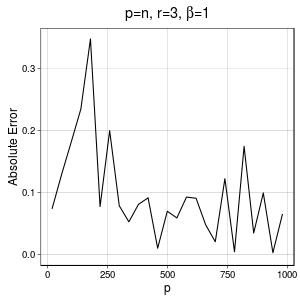
\includegraphics[height=6cm]{code/difference1.jpeg}
%    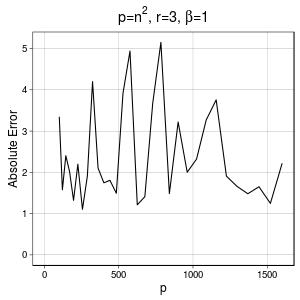
\includegraphics[height=6cm]{code/difference2.jpeg}\\
%    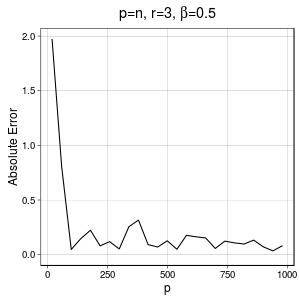
\includegraphics[height=6cm]{code/difference3.jpeg}
%    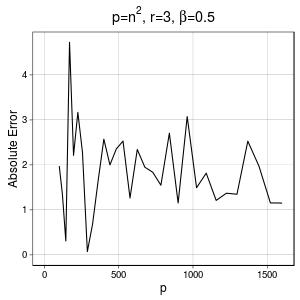
\includegraphics[height=6cm]{code/difference4.jpeg}\\
%    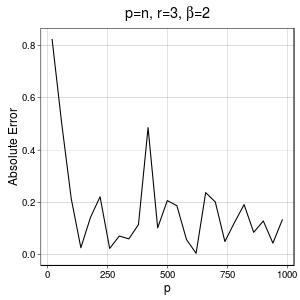
\includegraphics[height=6cm]{code/difference5.jpeg}
%    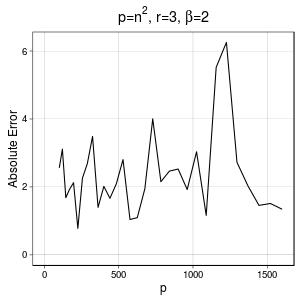
\includegraphics[height=6cm]{code/difference6.jpeg}\\
%    \caption{These are plots of $T_{\textrm{dif}}$ versus $p$. The first column and the second column are the case of $p=n$ and $p=n^2$, separately. The cases of $\beta=1,2,3$ are in the row $1,2,3$ separately. $r$ is set to be $3$ in all cases. }\label{fig:fig1}
%\end{figure}

First we simulate the level of the new test. We set factor number $r=2$.
Samples are repeatedly generated $1000$ times to calculate empirical level.
For comparison, we also give corresponding `oracle' level which is calculated by `statistic' ${T_1}/(\sigma^2\sqrt{2p\tau^2})$.
The results are listed in
Table~\ref{biaoge1}. From the results, we can find that for small $n$ and $p$, even oracle level is not satisfied.
Level of the new test is  a little inflated compared with oracle level. It performs better when $n$ is larger.

% latex table generated in R 3.3.1 by xtable 1.8-2 package
% Sun Jul 31 01:50:20 2016
\begin{table}[ht]

\caption{Test level simulation} 
\label{biaoge1}
    \vspace{3mm}
\centering
\begin{tabular}{rccccccc}
    \toprule
     &  & \multicolumn{2}{c}{$\beta$=0.5} & \multicolumn{2}{c}{$\beta$=1}& \multicolumn{2}{c}{$\beta$=2}   \\
    \cmidrule(r){3-4}
    \cmidrule(r){5-6}
    \cmidrule(r){7-8}
$n$ & $p$ & NEW & ORACLE & NEW & ORACLE & NEW & ORACLE \\ 
\midrule
300 & 200 & 0.075 & 0.062 & 0.079 & 0.062 & 0.074 & 0.070 \\ 
  300 & 400 & 0.074 & 0.065 & 0.061 & 0.044 & 0.046 & 0.040 \\ 
  300 & 600 & 0.058 & 0.041 & 0.070 & 0.052 & 0.071 & 0.055 \\ 
  300 & 800 & 0.066 & 0.047 & 0.071 & 0.052 & 0.062 & 0.048 \\ 
  600 & 200 & 0.061 & 0.055 & 0.052 & 0.051 & 0.058 & 0.056 \\ 
  600 & 400 & 0.051 & 0.048 & 0.051 & 0.042 & 0.059 & 0.051 \\ 
  600 & 600 & 0.061 & 0.058 & 0.056 & 0.054 & 0.051 & 0.047 \\ 
  600 & 800 & 0.053 & 0.046 & 0.060 & 0.050 & 0.056 & 0.048 \\ 
   \bottomrule
\end{tabular}
\end{table}




Next we simulate the empirical power of our test and~\cite{Chen2010A}'s test.
The simulation results of~\cite{Ma2015A} have showed that the level of the~\cite{Chen2010A}'s test can't be guaranteed when covariance is spiked.
To be fair, we use permutation method to compute critical value.
Permutation method can produce an exact test procedure, see~\cite{Lehmann}'s Example 15.2.2.\@
For $T_{CQ}$, note that permutation method only need it's main part, $\|\bar{X}_1-\bar{X}_2\|^2$, which is also the main part of~\cite{Bai1996Efiect} and~\cite{Ma2015A}'s method.
Thus, these methods all produce the same permutation test.
We plot the empirical power versus $\|\mu_1-\mu_2\|$ while other parameters hold constant.
The results are illustrated in figure~\ref{fig:fig2}.
From the results, we can find that when $\Sigma$ is spiked, the new test outperforms $T_{CQ}$ substantially; when $\Sigma$ is not spiked, the new test and $T_{CQ}$ are comparable.
\begin{figure}
    \centering 
    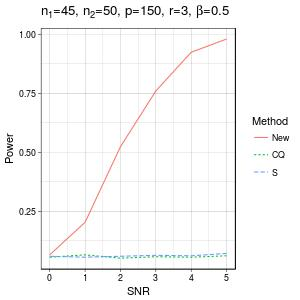
\includegraphics[height=6cm]{code/fig1.jpeg}
    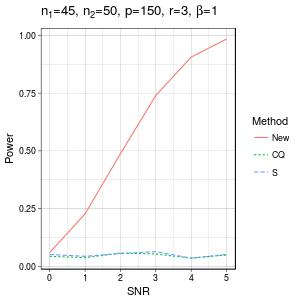
\includegraphics[height=6cm]{code/fig2.jpeg}
    \\
    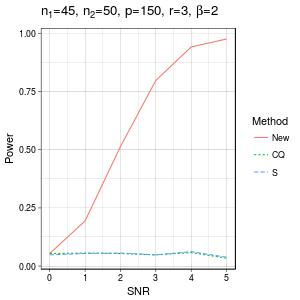
\includegraphics[height=6cm]{code/fig3.jpeg}
    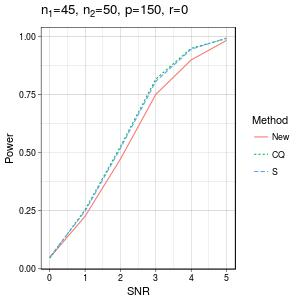
\includegraphics[height=6cm]{code/fig4.jpeg}
    \\
    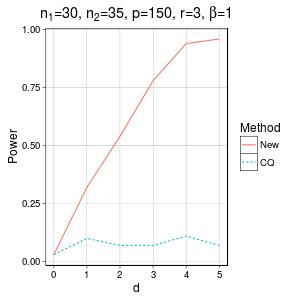
\includegraphics[height=6cm]{code/fig5.jpeg}
    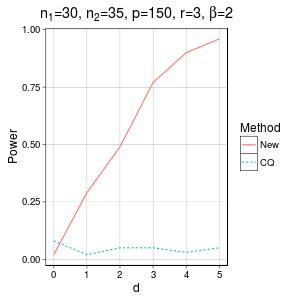
\includegraphics[height=6cm]{code/fig6.jpeg}
    \caption{Empirical power simulation. $\alpha$ is set to be $0.05$. $d$ is proportional to $\|\mu_1-\mu_2\|^2$. For each simulation, we do 50 permutations to determine critical value. We generate $100$ independent samples to compute empirical power. }\label{fig:fig2}
\end{figure}

%Permutation method is computation expensive. So when $p$ and $n$ are large, we simulate empirical power by asymptotic distribution. The results are illustrated in figure~\eqref{fig:fig3}.

%\begin{figure}\label{fig:fig3}
    %\centering 
    %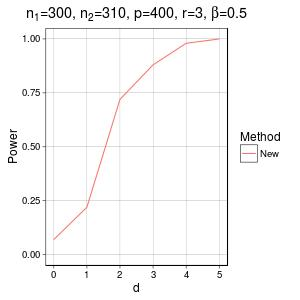
\includegraphics[height=6cm]{code/newfig1.jpeg}
    %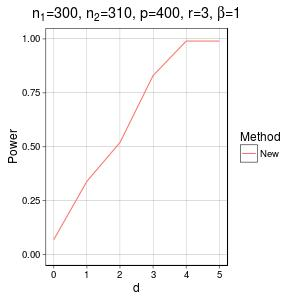
\includegraphics[height=6cm]{code/newfig2.jpeg}
    %\\
    %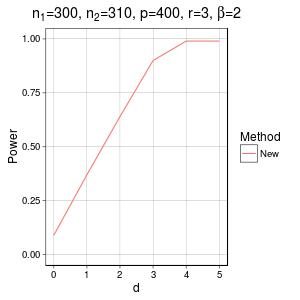
\includegraphics[height=6cm]{code/newfig3.jpeg}
    %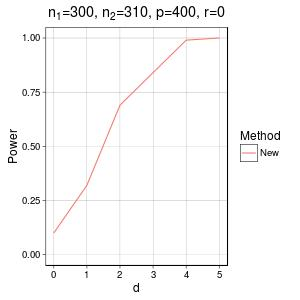
\includegraphics[height=6cm]{code/newfig4.jpeg}
    %\\
    %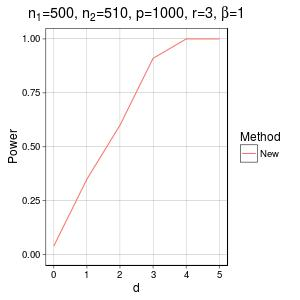
\includegraphics[height=6cm]{code/newfig5.jpeg}
    %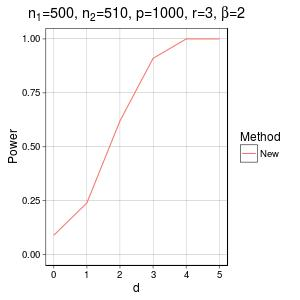
\includegraphics[height=6cm]{code/newfig6.jpeg}
    %\caption{Empirical Power (critical values are computed by asymptotic distribution)}\label{fig:fig3}
%\end{figure}

\subsection{Real data analysis}
In this section, we study the practical problem considered in~\cite{Ma2015A}.
The task is to test whether Monday stock returns are equal to those of other trading days on average.
Define an observation be the log return of stocks in a day.
Hence $p$ is the total number of stocks.
Let sample $1$ and sample $2$ be the observations on Monday and the other trading days, respectively.
Then we would like to test $H_0\, :\mu_1=\mu_2$ v.s. $H_1\,:\mu_1\neq \mu_2$.
We collected the data of $p=710$
 stocks of China
from 01/04/2013 to 12/31/2014. There are total $n_1=95$ Monday and $n_2=388$ other trading days. 

We assume $\Sigma_1=\Sigma_2$.
The first eigenvaule of $S$ is $0.14$, which is significantly larger than the others.
In fact, the second eigenvalue is $0.02$.
Hence there's clearly a spiked eigenvalue.
We set $r=1$ and perform our new test.
The $p$ value is $0.149$, which is obtained by $1000$ permutations.
Hence, the null hypothesis can not be rejected for $\alpha=0.05$.
We draw the same conclusion as~\cite{Ma2015A}.

\section{Conclusion remark}

This paper is concerned with the problem of testing the equality of means in the setting of high dimension and spiked covariance. We drop big variance terms from $T_{CQ}$ and obtain a new test statistic. The asymptotic normality of the new statistic is proved and the asymptotic power is given. %The new test outperforms $T_{CQ}$ substantially if the variance is spiked.
%We also generalize the test to unequal variance case.

In another paper,~\cite{Zhao2016A} proved that their test statistic can be written in the form of projection. Their simulation results showed that their test performs well under strong correlations.
Our work partially explains why their test performs well although the projections are slightly different. 

 Spiked covariance is an important correlation pattern and has been widely studied in terms of PCA\@.
 In PCA, authors focus on the principal subspace.
 However, in some circumstances, as our work have shown, the complement of principal subspace is more useful. 


Our theoretical results rely on the assumption $\sqrt{p}/n\to 0$. In the situation of small sample or very large $p$, the critical value of the new test can be determined by permutation method. Our simulation shows that the new test still performs well. It remains a theoretical interest to study the asymptotic behavior of permutation based test in these situations.



\section*{Appendix}

%\begin{lemma}\label{lemma1}
%    let $X$ be a $p$-dimensional random vector with distribution $N(0,\Sigma)$. Denote the spectral decomposition of $\Sigma$ by $\Sigma =\sum_{i=1}^p \lambda_i p_i p_i^T$ with $\lambda_1\geq \cdots \geq \lambda_p$. Then $X^T p_i p_i^T X$ is stochastically larger than $X^T p_j p_{j}^T X$ for $i<j$.
%\end{lemma}
%\begin{proof}[\textbf{Proof}]
%    The lemma is established immediately once we note that $X^T p_i p_i^T X/\sqrt{\lambda_i}$ is distributed as $\chi^2$ distribution with freedom $1$.
%\end{proof}

\begin{lemma}[Weyl's inequality]
Let $H$ and $P$ be two symmetric matrices and $M=H+P$. If $j+k-n\geq i\geq r+s-1$, we have
\begin{equation*}
\lambda_j(H)+\lambda_k(P)\leq \lambda_i(M) \leq \lambda_r(H)+\lambda_s(P).
\end{equation*}
\end{lemma}
\begin{corollary}\label{WeylCor}
    Let $H$ and $P$ be two symmetric matrices and $M=H+P$. If $\mathrm{rank}(P)< k$, then
    \begin{equation*}
        \lambda_k(M)\leq \lambda_1(H).
    \end{equation*}
\end{corollary}


\begin{lemma}[Convergence rate of principal space estimation]\label{conRateLemma}
    Under the Assumption~\ref{balance}-\ref{theModel2}, we have
\begin{equation*}
E\|\hat{V}\hat{V}^T-VV^T\|^2_F =O(\frac{p}{p^{\beta}n}).
\end{equation*}
\end{lemma}


\begin{proof}[\textbf{Proof}]
    Theorem 5 of~\cite{Cai2012Sparse} asserts that sample principal subspace $\hat{V}\hat{V}^T$ is a minimax rate estimator of $VV^T$, namely, it reaches the minimax convergence rate
    \begin{equation}\label{xiaopianpian}
         E\|\hat{V}\hat{V}^T-VV^T\|^2_F\asymp r\wedge (p-r)\wedge \frac{r(p-r)}{(n_1+n_2-2)h(\lambda)}
    \end{equation}
    as long as the right hand side tends to $0$. Here $h(\lambda)=\frac{\lambda^2}{\lambda+1}$. In model of Assumption~\ref{theModel},  $r$ is fixed, $\lambda=cp^\beta$.
    It's obvious that the right hand side of~\eqref{xiaopianpian} is of order ${p^{1-\beta}}/{n}$.
    We note that it is assumed $\beta\geq \frac{1}{2}$ in Assumption~\ref{orderOfBeta}, together with ${\sqrt{p}}/{n}\to 0$ we have
    ${p^{1-\beta}}/{n}\to 0$. Hence
    $\hat{V}\hat{V}^T$ reaches the convergence rate.

\end{proof}
\begin{lemma}[Bai-Yin's law]\label{baiyin}
    Suppose $B_n=\frac{1}{q} Z Z^T$ where $Z$ is $p\times q$ random matrix composed of i.i.d.\ random variables with zero mean, unit variance and finite fourth moment.
    As $q\to \infty$ and $\frac{p}{q}\to c\in [0,\infty)$, the largest and smallest non-zero eigenvalues of $B_n$ converge almost surely to ${(1+\sqrt{c})}^2$ and $(1-\sqrt{c})^2$, respectively.
\end{lemma}
\begin{remark}
    Lemma~\ref{baiyin} is known as the Bai-Yin's law (\cite{bai1993limit}). As in Remark $1$ of~\cite{bai1993limit}, the smallest non-zero eigenvalue is the $p-q+1$ smallest eigenvalue of $B$ for $c>1$.
\end{remark}
\begin{corollary}\label{maxEigen}
    Suppose that $W_n$ is a $p \times p$ matrix distributed as $\mathrm{Wishart}_p(n,I_{p})$. Then as $n\to \infty$,
    $$
        \lambda_1(W_n)=O_P(\max(n,p)).
    $$
\end{corollary}
\begin{proof}[\textbf{Proof}]
    Since $[0,+\infty]$ is compact, for every subsequance $\{n_{k}\}$ of $\{n\}$, there is a further subsequance $\{n_{k_l}\}$ along which $p/n\to c\in [0,+\infty]$.

    If $c\in [0,+\infty)$, by Lemma~\ref{baiyin}, we have that
    $$
    \frac{\lambda_1(W_{n_{k_l}})}{n_{k_l}}\xrightarrow{P}{(1+c)}^2.
    $$
    Hence the conclusion holds along this subsequance. If $c=+\infty$, suppose $W_n=Z_n Z_n^T$ where $Z_n$ is a $p\times n$ matrix with all elements distributed as $N(0,1)$. Then
    $$
    \frac{\lambda_1(W_{n_{k_l}})}{p}=\frac{Z_{n_{k_l}}^T Z_{n_{k_l}}}{p}\xrightarrow{P} 1,
    $$
    by Lemma~\ref{baiyin}, which proves the conclusion along the subsequance. Now the conclusion holds by a standard subsequance argument.
\end{proof}


\begin{lemma}\label{quadraticFormCLT}
    Suppose $X_{n}$ is a $k_n$ dimensional standard normal random vector and $A_n$ is a $k_n\times k_n$ symmetric matrix. Then a necessary and sufficient condition for
    \begin{equation}\label{quadratic}
        \frac{X_n^T A_n X_n-\mathrm{E}X_n^T A_n X_n}{{[\mathrm{Var}(X_n^T A_n X_n)]}^{1/2}}\xrightarrow{\mathcal{L}}N(0,1)
    \end{equation}
    is that
    \begin{equation}\label{quadraticEigen}
        \frac{\lambda_{\max}(A_n^2)}{\mathrm{tr}(A_n^2)}\to 0.
    \end{equation}
\end{lemma}
\begin{remark}
This lemma is from the Example 5.1 of~\cite{jiang1996reml}. Here we give a proof by characteristic function.
\end{remark}
\begin{proof}
    Let $\lambda_1(A_n)\geq\cdots\geq \lambda_{k_n}(A_n)$ be the eigenvalues of $A_n$, then 
    \begin{equation}
        \frac{X_n^T A_n X_n-\mathrm{E}X_n^T A_n X_n}{{[\mathrm{Var}(X_n^T A_n X_n)]}^{1/2}}=\sum_{i=1}^{k_n}\frac{\lambda_i(A_n)}{{\big[2\mathrm{tr}(A_n^2)\big]}^{1/2}}(Z_{ni}^2-1),
    \end{equation}
    where $Z_{ni}$'s ($i=1,\ldots,k_n$) are independent standard normal random variables.

    If~\ref{quadraticEigen} holds, then
    \begin{equation*}
        \begin{aligned}
            &\sum_{i=1}^{k_n}\mathrm{E}\Big[\frac{\lambda_i^2(A_n)}{2\mathrm{tr}(A_n^2)}{(Z_{ni}^2-1)}^2\Big\{\frac{\lambda_i^2(A_n)}{2\mathrm{tr}(A_n^2)}{(Z_{ni}^2-1)}^2\geq \epsilon\Big\}\Big]\\
            \leq&\sum_{i=1}^{k_n}
            \frac{\lambda_i^2(A_n)}{2\mathrm{tr}(A_n^2)}
            \mathrm{E}\Big[{(Z_{n1}^2-1)}^2\Big\{\frac{\lambda_{\max}(A_n^2)}{2\mathrm{tr}(A_n^2)}{(Z_{n1}^2-1)}^2\geq \epsilon\Big\}\Big]\\
            =&
            \frac{1}{2}\mathrm{E}\Big[{(Z_{n1}^2-1)}^2\Big\{\frac{\lambda_{\max}(A_n^2)}{2\mathrm{tr}(A_n^2)}{(Z_{n1}^2-1)}^2\geq \epsilon\Big\}\Big]\to 0.
        \end{aligned}
    \end{equation*}
    Hence~\ref{quadratic} follows by Lindeberg's central limit theorem.

    Conversely, if~\ref{quadratic} holds, we will prove that there is a subsequence of $\{n\}$ along which~\ref{quadraticEigen} holds. Then~\ref{quadraticEigen} will hold by a standard contradiction argument. 

    Denote $c_{ni}=\lambda_i(A_n)/{\big[2\mathrm{tr}(A_n^2)\big]}^{1/2}$ ($i=1,\ldots,k_n$), we have $c_{ni}\in[-\sqrt{2}/2,\sqrt{2}/2]$.
    Since~\ref{quadratic} holds, the characteristic function of
        $
        \sum_{i=1}^{k_n}c_{ni}(Z_{ni}^2-1)
    $
    converges to $\exp(-t^2/2)$ for every $t$. For $t\in (-1,1)$, we have
    \begin{equation*}
        \begin{aligned}
            &\log \mathrm{E}\exp{\big(it \sum_{j=1}^{k_n}c_{nj}(Z_{nj}^2-1)\big)}
            =
            -i(\sum_{j=1}^{k_n}c_{nj})t-
            \frac{1}{2}\sum_{j=1}^{k_n}\log(1-i2c_{nj}t)\\
            =&
            -i(\sum_{j=1}^{k_n}c_{nj})t+
            \frac{1}{2}\sum_{j=1}^{k_n}\sum_{l=1}^{+\infty}\frac{1}{l}{(i2c_{nj}t)}^l
            =
            -i(\sum_{j=1}^{k_n}c_{nj})t+
            \frac{1}{2}\sum_{l=1}^{+\infty}\Big[\sum_{j=1}^{k_n}{(c_{nj})}^l\Big]\frac{1}{l}{(i2t)}^l\\
            =&-\frac{1}{2}t^2+
            \frac{1}{2}\sum_{l=3}^{+\infty}\Big[\sum_{j=1}^{k_n}{(c_{nj})}^l\Big]\frac{1}{l}{(i2t)}^l.
        \end{aligned}
    \end{equation*}
    Denote $b_{nl}=\sum_{j=1}^{k_n}{(c_{nj})}^l$, $n=1,2,\cdots$ and $l=3,4,\cdots$. For $l\geq 3$, $\big|\sum_{j=1}^{k_n}{(c_{nj})}^l\big|\leq \big|\sum_{j=1}^{k_n}{(c_{nj})}^2\big|=1/2$.
    By Helly's selection theorem, there's a subsequence of $\{n\}$ along which $\lim_{n\to \infty}b_{nl}=b_l$ exists for every $l$.
    Apply dominated convergence theorem to this subsequence we have
            $\log \mathrm{E}\exp{\big(it \sum_{j=1}^{k_n}c_{nj}(Z_{nj}^2-1)\big)}\to
            -\frac{1}{2}t^2+
            \frac{1}{2}\sum_{l=3}^{+\infty}b_l\frac{1}{l}{(i2t)}^l$ for $t\in(-1/2,1/2)$.
            By the property of power series, we have $b_l=0$ for $l\geq 3$. Then~\ref{quadraticEigen} follows by noting that $b_{n4}\geq \max_j{(c_{nj})}^4$.
\end{proof}




The rest of the Appendix is devoted to the proof of propositions and theorems in the paper.

\begin{proof}[\textbf{Proof of Proposition~\ref{newIf}}]
    We first note that~\eqref{chenscondition} is equivalent to
\begin{equation}\label{ChenMaxEigen}
    \frac{\lambda_{\max}^2(\Sigma)}{\mathrm{tr}\Sigma^2}\to 0.
\end{equation}

    Let $Z_{k,i}=\Sigma^{-1/2}X_{k,i}$. Then $Z_{k,i}\sim N_p(0,I_{p})$.
    Denote 
    $$Z={(Z_{1,1}^T,\ldots,Z_{1,n_1}^T,Z_{2,1}^T,\ldots,Z_{2,n_2}^T)}^T.$$
    Note that $T_{CQ}$ is a quadratic form of $Z$ and can be written as
        $$
        T_{CQ}=Z^T \big( B_n\otimes \Sigma \big) Z,
        $$
    where 
    \begin{equation*}
        B_n=\begin{pmatrix}
            \frac{1}{n_1(n_1-1)}(n_1\gamma_1\gamma_1^T-I_{n_1})&
            -\frac{1}{\sqrt{n_1 n_2}}\gamma_1 \gamma_2^T\\
            -\frac{1}{\sqrt{n_1 n_2}}\gamma_2 \gamma_1^T&
            \frac{1}{n_2(n_2-1)}(n_2\gamma_2\gamma_2^T-I_{n_2})\\
        \end{pmatrix},
    \end{equation*}
    $\gamma_1$ is an $n_1$ dimensional vector with all elements equal to $1/\sqrt{n_1}$ and $\gamma_2$ is an $n_2$ dimensional vector with all elements equal to $1/\sqrt{n_2}$.

    By direct calculation, it can be seen that $B_n$'s eigenvalues are $-1/n_1(n_1-1)$, $-1/n_2(n_2-1)$, $(n_1+n_2)/n_1 n_2$ and $0$ with multiplicities $n_1-1$, $n_2-1$, $1$ and $1$ respectively.
    The eigenspace corresponding to $-1/n_1(n_1-1)$ is
    \begin{equation*}
        \{{(\eta^T,\underbrace{0,\ldots,0}_{n_2})}^T|\, \textrm{$\eta\in \mathbb{R}^{n_1}$ and $\eta^T \gamma_1=0$}\}.
    \end{equation*}
    The eigenspace corresponding to $-1/n_2(n_2-1)$ is
    \begin{equation*}
        \{{(\underbrace{0,\ldots,0}_{n_1},\eta^T)}^T| \, \textrm{$\eta\in\mathbb{R}^{n_2}$ and $\eta^T \gamma_2=0$}\}.
    \end{equation*}
    The eigenvector corresponding to $(n_1+n_2)/n_1n_2$ is
    \begin{equation*}
        {\Big(-\sqrt{\frac{n_2}{n_1+n_2}}\gamma_1^T, \sqrt{\frac{n_1}{n_1+n_2}}\gamma_2^T\Big)}^T.
    \end{equation*}
    The eigenvector corresponding to $0$ is
    \begin{equation*}
        {\Big(\sqrt{\frac{n_1}{n_1+n_2}}\gamma_1^T, \sqrt{\frac{n_2}{n_1+n_2}}\gamma_2^T\Big)}^T.
    \end{equation*}
It follows that 
    \begin{equation*}
        \mathrm{tr}{(B_n\otimes \Sigma)}^2=\mathrm{tr}(B_n^2)\mathrm{tr}\Sigma^2=(\frac{1}{n_1(n_1-1)}+\frac{1}{n_1(n_1-1)}+\frac{2}{n_1 n_2})\mathrm{tr}\Sigma^2.
    \end{equation*}
And
    \begin{equation*}
        \lambda_{\max}\Big({(B_n\otimes \Sigma)}^2\Big)=\lambda_{\max}(B_n^2)\lambda_{\max}(\Sigma^2)={\Big(\frac{1}{n_1}+\frac{1}{n_2}\Big)}^2\lambda_{\max}(\Sigma^2).
    \end{equation*}
    The theorem follows by Lemma~\ref{quadraticFormCLT}.
\end{proof}



\begin{proof}[\textbf{Proof of Proposition~\ref{oracleTheorem}}]
    Let $Y_{k,i}=\tilde{V}^T (X_{k,i}-\mu_k)$, $i=1,\ldots,n_k$, $k=1,2$.
    Then $Y_{k,i}\sim N(\tilde{V}^T\mu_k,\sigma^2 I_{p-r})$.
    Let $\bar{Y}_1$ and $\bar{Y}_2$ be the sample means of $\{Y_{1,i}\}_{i=1}^{n_1}$ and $\{Y_{2,i}\}_{i=1}^{n_2}$ respectively. 
    Then
    \begin{equation}\label{prop1eq1}
        \begin{aligned}
            &\|\tilde{V}^T(\bar{X}_1-\bar{X}_2)\|^2
            =\|\tilde{V}^T(\mu_1-\mu_2)+(\bar{Y}_1-\bar{Y}_2)\|^2\\
            =&\|\tilde{V}^T(\mu_1-\mu_2)\|^2+\|\bar{Y}_1-\bar{Y}_2\|^2+
            2{(\mu_1-\mu_2)}^T\tilde{V}(\bar{Y}_1-\bar{Y}_2)\\
            =&\|\tilde{V}^T(\mu_1-\mu_2)\|^2+\|\bar{Y}_1-\bar{Y}_2\|^2+
            o_P(\frac{\sqrt{p}}{n}).
        \end{aligned}
    \end{equation}
    The last equality holds since
    \begin{equation*}
        \begin{aligned}
            &2{(\mu_1-\mu_2)}^T\tilde{V}(\bar{Y}_1-\bar{Y}_2)\sim N(0,4\sigma^2 \tau \|\tilde{V}^T(\mu_1-\mu_2)\|^2)\\
            =& O_P(\sqrt{\tau}\|\tilde{V}^T(\mu_1-\mu_2)\| )=o_P(\frac{\sqrt{p}}{n}).
        \end{aligned}
    \end{equation*}
    For $k=1,2$, we have
    %${n_k^{-1}} \tilde{V}^T S_k \tilde{V}\sim
    %\frac{\sigma^2}{n_k(n_k-1)}\operatorname{Wishart}_{p-r}(n_k-1,I_{p-r})
    %$, $k=1,2$.
    %Then 
    \begin{equation*}
        \begin{aligned}
            &\frac{1}{n_k} \mathrm{tr}(\tilde{V}^T S_k \tilde{V})\sim \frac{\sigma^2}{n_k(n_k-1)}\chi^2_{(p-r)(n_k-1)}\\
            =&
            \sigma^2\frac{p-r}{n_k}(1+O_P(\frac{1}{\sqrt{(p-r)(n_k-1)}})),
        \end{aligned}
    \end{equation*}
    where the last equality comes from central limit theorem. It follows that
    \begin{equation}\label{prop1eq2}
        \begin{aligned}
            &\frac{1}{n_1} \mathrm{tr}(\tilde{V}^T S_1 \tilde{V})+
            \frac{1}{n_2} \mathrm{tr}(\tilde{V}^T S_2 \tilde{V})=\sigma^2 \tau (p-r)+o_P(\frac{\sqrt{p}}{n}).
        \end{aligned}
    \end{equation}

    Equation~\eqref{prop1eq1} and~\eqref{prop1eq2} imply that
    \begin{equation}
        \begin{aligned}
            \frac{T_1-\|\tilde{V}^T(\mu_1-\mu_2)\|^2}{\sigma^2\sqrt{2\tau^2 p}}
            =
            \frac{\|\bar{Y}_1-\bar{Y}_2\|^2-
                \sigma^2 \tau (p-r)}{\sigma^2\sqrt{2\tau^2 p}}
                +o_P(1).
        \end{aligned}
    \end{equation}
    Since
$\|\tilde{V}^T(\bar{Z}_1-\bar{Z}_2)\|^2\sim \sigma^2\tau\chi^2_{p-r}$,
the proposition follows by central limit theorem.
\end{proof}



\begin{proof}[\textbf{Proof of Proposition~\ref{varianceEstimation}}]
    Note that $(n-2)S\sim \mathrm{Wishart}_p (n-2,\Sigma)$.
    Denote by $\Sigma=UEU^T$ the spectral decomposition of $\Sigma$, where $U=(V,\tilde{V})$ is an orthogonal matrix and $E=\mathrm{diag}(\lambda_1+\sigma^2,\ldots,\lambda_r+\sigma^2,\sigma^2,\ldots,\sigma^2)$.
    Let $Z$ be a $p\times (n-2)$ random matrix with all elements i.i.d.\ distributed as $N(0,1)$, then
    $$
        S\sim \frac{1}{n-2} U E^{1/2} Z Z^T E^{1/2} U^T.
    $$
    Thus,
    \begin{equation*}
        \begin{aligned}
            \hat{\sigma}^2\sim
            \frac{1}{(p-r)(n-2)}\sum_{i=r+1}^p \lambda_i (U E^{1/2} Z Z^T E^{1/2} U^T)
            =
            \frac{1}{(p-r)(n-2)}\sum_{i=r+1}^{n-2} \lambda_i ( Z^T E Z).
        \end{aligned}
    \end{equation*}
    Denote $Z={(Z_{(1)}^T,Z_{(2)}^T)}^T$, where $Z_{(1)}$ and $Z_{(2)}$ are the first $r$ rows and last $p-r$ rows of $Z$. We have
    $$
    Z^T E Z =Z_{(1)}^T (\Lambda +\sigma^2 I_r) Z_{(1)}+\sigma^2 Z_{(2)}^T Z_{(2)}.
    $$
 The first term is of rank $r$. By Weyl's inequality, we have
    $$
    \sigma^2\lambda_i(Z_{(2)}^T Z_{(2)}) \leq \lambda_i(Z^T E Z)\leq
    \sigma^2\lambda_{i-r}(Z_{(2)}^T Z_{(2)}),
    \quad
    \textrm{$i=r+1,\ldots, n-2$}.
    $$
    Thus,
    $$
    \sigma^2\sum_{i=r+1}^{n-2}\lambda_i(Z_{(2)}^T Z_{(2)}) \leq \sum_{i=r+1}^{n-2}\lambda_i(Z^T E Z)\leq
    \sigma^2\sum_{i=1}^{n-r-2}\lambda_{i}(Z_{(2)}^T Z_{(2)}).
    $$
     It follows that
     \begin{equation*}
         \begin{aligned}
             &\Big|\frac{1}{(p-r)(n-2)}\sum_{i=r+1}^{n-2}\lambda_i(Z^T E Z)-
    \frac{1}{(p-r)(n-2)} \sigma^2\sum_{i=1}^{n-2}\lambda_{i}(Z_{(2)}^T Z_{(2)})\Big|
             \\
             \leq & r\sigma^2\frac{1}{(p-r)(n-2)} \lambda_1 (Z_{(2)}^T Z_{(2)}).
         \end{aligned}
     \end{equation*}
    By Corollary~\ref{maxEigen}, $\lambda_1 (Z_{(2)}^T Z_{(2)})=O_P(\max(n,p))$. 
    Thus,
     \begin{equation*}
         \begin{aligned}
             &\frac{1}{(p-r)(n-2)}\sum_{i=r+1}^{n-2}\lambda_i(Z^T E Z)\\
             =&
    \frac{1}{(p-r)(n-2)} \sigma^2\sum_{i=1}^{n-2}\lambda_{i}(Z_{(2)}^T Z_{(2)})
             +O_P(\frac{\max(n,p)}{np})\\
             =&
             \frac{1}{(p-r)(n-2)} \sigma^2\mathrm{tr}(Z_{(2)}^T Z_{(2)})
             +O_P(\frac{\max(n,p)}{np})\\
             =&
             \sigma^2
                +O_P(\frac{1}{\sqrt{np}})
             +O_P(\frac{\max(n,p)}{np}).\\
         \end{aligned}
     \end{equation*}
     The last equality comes from central limit theorem.
The theorem follows by noting that
$$
    O_{P}(\frac{1}{\sqrt{np}})=O_P(\frac{\sqrt{np}}{np})= O_P(\frac{\max (n,p)}{np}).
$$
\end{proof}



% proof of space estimation theorem
\begin{proof}[\textbf{Proof of Theorem~\ref{myPanpan}}]

    Note that $\mathrm{tr}(\hat{\tilde{V_k}}^T S_k\hat{\tilde{V_k}})=\sum_{i=r+1}^p \lambda_i(S_k)$, $k=1,2$.
    Similar to Proposition~\ref{varianceEstimation}, we have $\mathrm{tr}(\hat{\tilde{V_k}}^T S_k\hat{\tilde{V_k}})=(p-r)\sigma^2+O_P({\max(n,p)}/{n})$, $k=1,2$.
    Then
\begin{equation*}
        \frac{T_2-\|\tilde{V}^T(\mu_1-\mu_2)\|^2}{\sigma^2\sqrt{2\tau^2 p}}
        =
        \frac{\|\hat{\tilde{V}}^T(\bar{X}_1-\bar{X}_2)\|^2-\|\tilde{V}^T(\mu_1-\mu_2)\|^2
        -\sigma^2\tau (p-r)
        }{\sigma^2\sqrt{2\tau^2 p}}
        +O_P(\frac{\max(n,p)}{n\sqrt{p}}).
\end{equation*}
    By Assumption~\ref{pAndN}, ${n^{-1}p^{-1/2}}{\max(n,p)}=\max({p}^{-1/2},{p}^{1/2}/n)\to 0$.
    Note that
\begin{equation*}
    \begin{aligned}
        &\frac{\|\hat{\tilde{V}}^T(\bar{X}_1-\bar{X}_2)\|^2-\|\tilde{V}^T(\mu_1-\mu_2)\|^2
        -\sigma^2\tau (p-r)
        }{\sigma^2\sqrt{2\tau^2 p}}
        \\
        =&\frac{1}{\sigma^2\sqrt{2\tau^2 p}}\Big(
        \|\hat{\tilde{V}}^T\big((\bar{X}_1-\mu_1)-(\bar{X}_2-\mu_2)\big)\|^2-\sigma^2 \tau (p-r)+\\
        &2{(\mu_1-\mu_2)}^T \hat{\tilde{V}}\hat{\tilde{V}}^T\big((\bar{X}_1-\mu_1)-(\bar{X}_2-\mu_2)\big)
        +\|\hat{\tilde{V}}^T(\mu_1-\mu_2)\|^2-\|\tilde{V}^T(\mu_1-\mu_2)\|^2
        \Big).
    \end{aligned}
\end{equation*}
Let 
\begin{align*}
    P_1&=\|\hat{\tilde{V}}^T\big((\bar{X}_1-\mu_1)-(\bar{X}_2-\mu_2)\big)\|^2-\sigma^2 \tau (p-r),\\
    P_2&=2{(\mu_1-\mu_2)}^T \hat{\tilde{V}}\hat{\tilde{V}}^T\big((\bar{X}_1-\mu_1)-(\bar{X}_2-\mu_2)\big),\\
    P_3&=\|\hat{\tilde{V}}^T(\mu_1-\mu_2)\|^2-\|\tilde{V}^T(\mu_1-\mu_2)\|^2.
\end{align*}
To prove the theorem, it suffices to show that
$$
    \frac{P_1}{\sigma^2\sqrt{2\tau^2 p}}\xrightarrow{\mathcal{L}} N(0,1),
    \quad
    \frac{P_2}{\sigma^2\sqrt{2\tau^2 p}}\xrightarrow{P} 0
    \quad
    \textrm{and}
    \quad
    \frac{P_3}{\sigma^2\sqrt{2\tau^2 p}}\xrightarrow{P}0.
    $$
    We first deal with $P_2$.
    To proves the convergence in probability, we only need to prove the convergence in $L^2$.
    Note that $\bar{X}_1$, $\bar{X}_2$, and $S$ are mutually independent and $\hat{\tilde{V}}\hat{\tilde{V}}^T$ only depends on $S$. Thus
    \begin{equation*}
        \begin{aligned}
            &\mathrm{E} P_2^2
            =
            \mathrm{E}[\mathrm{E} P_2^2|S]= 4\tau \mathrm{E}[{(\mu_1-\mu_2)}^T \hat{\tilde{V}}\hat{\tilde{V}}^T\Sigma \hat{\tilde{V}}\hat{\tilde{V}}^T(\mu_1-\mu_2)]\\
            \leq &
             4\tau\mathrm{E}[\lambda_1(\hat{\tilde{V}}^T\Sigma \hat{\tilde{V}}) {(\mu_1-\mu_2)}^T \hat{\tilde{V}}\hat{\tilde{V}}^T(\mu_1-\mu_2)]
            \leq 
             4\tau\|\mu_1-\mu_2\|^2
             \mathrm{E}[\lambda_1(\hat{\tilde{V}}^T\Sigma \hat{\tilde{V}}) ]\\
             =&
             O(\frac{\sqrt{p}}{n^2})
             \mathrm{E}[\lambda_1(\hat{\tilde{V}}^T (V\Lambda V^T +\sigma^2 I_p) \hat{\tilde{V}})]
             \leq 
             O(\frac{\sqrt{p}}{n^2})
             \big(\kappa p^{\beta}\mathrm{E}[\lambda_1(\hat{\tilde{V}}^T VV^T  \hat{\tilde{V}})]+\sigma^2\big).\\
        \end{aligned}
    \end{equation*}
    By the relationship
    \begin{equation*}
        \begin{aligned}
\lambda_1(\hat{\tilde{V}}^T VV^T  \hat{\tilde{V}})
            \leq
            \mathrm{tr}(\hat{\tilde{V}}^T VV^T  \hat{\tilde{V}})
            =
            \frac{1}{2}\|VV^T-\hat{V}\hat{V}^T\|^2_F
        \end{aligned}
    \end{equation*}
    and Lemma~\ref{conRateLemma}, we have that
    \begin{equation*}
        \begin{aligned}
            &\mathrm{E} P_2^2
             =
             O(\frac{\sqrt{p}}{n^2})
             \big(O(\frac{p}{n})+\sigma^2\big)
             =o(\frac{p}{n^2}).
        \end{aligned}
    \end{equation*}
    Next we deal with $P_3$. To prove the convergence in probability, we prove the convergence in $L^1$.
    \begin{equation*}
        \begin{aligned}
            &\mathrm{E}|P_3|=
            \mathrm{E}\big|{(\mu_1-\mu_2)}^T(\hat{\tilde{V}}\hat{\tilde{V}}^T-\tilde{V}\tilde{V}^T)(\mu_1-\mu_2)\big|
            \leq 
            \|\mu_1-\mu_2\|^2\mathrm{E}\|\hat{\tilde{V}}\hat{\tilde{V}}^T-\tilde{V}\tilde{V}^T\|\\
            =& 
            \|\mu_1-\mu_2\|^2\mathrm{E}\|\hat{V}\hat{V}^T-VV^T\|
            \leq 
            \|\mu_1-\mu_2\|^2\sqrt{\mathrm{E}\|\hat{V}\hat{V}^T-VV^T\|^2}\\
            \leq &
            \|\mu_1-\mu_2\|^2\sqrt{\mathrm{E}\|\hat{V}\hat{V}^T-VV^T\|^2_F}
            =O(\frac{\sqrt{p}}{n})\sqrt{O(\frac{p}{p^{\beta}n})}=o(\frac{\sqrt{p}}{n}).
        \end{aligned}
    \end{equation*}

    Now we prove the asymptotic normality of $P_1$. To make clear the sense of convergence, we need a metric for weak convergence. For two distribution function $F$ and $G$, the Levy metric $\rho$ of $F$ and $G$ is defined as
    $$
   \rho(F,G) =\inf\{\epsilon:F(x-\epsilon)-\epsilon\leq G(x)\leq F(x+\epsilon)+\epsilon\quad \textrm{for all $x$}\}.
    $$
    It's well known that $\rho(F_n,F)\to 0$ if and only if $F_n\xrightarrow{\mathcal{L}}F$.

    The conditional distribution of
    $\hat{\tilde{V}}^T\big((\bar{X}_1-\mu_1)-(\bar{X}_2-\mu_2)\big)$ given $S$ is $N(0,\tau \hat{\tilde{V}}^T\Sigma\hat{\tilde{V}})$.
It can be seen that 
$$\tau^{-1}\big\|\hat{\tilde{V}}^T\big((\bar{X}_1-\mu_1)-(\bar{X}_2-\mu_2)\big)\big\|^2
\sim
    \sum_{i=1}^{p-r} \lambda_i(\hat{\tilde{V}}^T\Sigma\hat{\tilde{V}})\xi_i^2,
    $$
where $\{\xi_i\}_{i=1}^{p-r}$ are i.i.d. standard normal random variables which are independent of $\hat{\tilde{V}}$.
    Note that
    $$
     \lambda_1(\hat{\tilde{V}}^T\Sigma\hat{\tilde{V}})\leq 
    \frac{1}{2}\kappa p^\beta \|VV^T -\hat{V}\hat{V}^T\|^2_F+\sigma^2.
    $$
    Hence $\lambda_i(\hat{\tilde{V}}^T\Sigma\hat{\tilde{V}})=O_P({p}/{n}+1)$, $i=1,\ldots,r$.
    Moreover, by Weyl's inequality,
    $
    \lambda_i(\hat{\tilde{V}}^T\Sigma\hat{\tilde{V}})=\sigma^2
    $, $i=r+1,\ldots,p-r$.
    Therefore
\begin{equation}\label{traceA1}
\mathrm{tr}(\hat{\tilde{V}}^T\Sigma\hat{\tilde{V}})^2=
    {\big(\frac{p}{n}+1\big)}^2O_P(1)
    +
    (p-2r)\sigma^4
    =p\sigma^4(1+o_P(1)).
\end{equation}

    It follows that
\begin{equation}\label{inProbC}
        \frac{\lambda_1^2(\hat{\tilde{V}}^T\Sigma\hat{\tilde{V}})}{\mathrm{tr}(\hat{\tilde{V}}^T\Sigma\hat{\tilde{V}})^2}
        =O_P\Big(\frac{{(p/n+1)}^2}{p}\Big)=o_P(1).
\end{equation}
Then for every subsequence of $\{n\}$, there's a further subsequence along which~\eqref{inProbC} holds almost surely.
By Lemma~\ref{quadraticFormCLT}, for every subsequence of $\{n\}$, there's a further subsequence along which we have
\begin{equation}\label{aseq}
\rho\Big(\mathcal{L}\Big(\frac{\|\hat{\tilde{V}}^T\big((\bar{X}_1-\mu_1)-(\bar{X}_2-\mu_2)\big)\|^2-\tau\mathrm{tr}(\hat{\tilde{V}}^T\Sigma\hat{\tilde{V}})}{\sqrt{2\tau^2\mathrm{tr}(\hat{\tilde{V}}^T\Sigma\hat{\tilde{V}})^2}}\Big|S\Big),N(0,1)\Big)\xrightarrow{a.s.} 0.
\end{equation}
It means that~\eqref{aseq} tends to $0$ in probability.
%$$
%\rho\Big(\mathcal{L}\Big(\frac{\|\hat{\tilde{V}}^T\big((\bar{X}_1-\mu_1)-(\bar{X}_2-\mu_2)\big)\|^2-\tau\mathrm{tr}(\hat{\tilde{V}}^T\Sigma\hat{\tilde{V}})}{\sqrt{2\tau^2\mathrm{tr}(\hat{\tilde{V}}^T\Sigma\hat{\tilde{V}})^2}}\Big|S\Big),N(0,1)\Big)\xrightarrow{P} 0.
%$$
It can be seen that the weak convergence also holds unconditionally.
$$
\frac{\|\hat{\tilde{V}}^T\big((\bar{X}_1-\mu_1)-(\bar{X}_2-\mu_2)\big)\|^2-\tau\mathrm{tr}(\hat{\tilde{V}}^T\Sigma\hat{\tilde{V}})}{\sqrt{2\tau^2\mathrm{tr}(\hat{\tilde{V}}^T\Sigma\hat{\tilde{V}})^2}}\xrightarrow{\mathcal{L}}N(0,1).
$$

Similar to~\eqref{traceA1} we have
\begin{equation}\label{traceA2}
    \mathrm{tr}(\hat{\tilde{V}}^T\Sigma\hat{\tilde{V}})=(p-r)\sigma^2\big(1+O_P\big(\frac{1}{n}+\frac{1}{p}\big)\big).
\end{equation}
By~\eqref{traceA1},~\eqref{traceA2} and Slulsk's theorem,
$$
\frac{\|\hat{\tilde{V}}^T\big((\bar{X}_1-\mu_1)-(\bar{X}_2-\mu_2)\big)\|^2-\sigma^2\tau(p-r) }{\sigma^2\sqrt{2\tau^2 p}}\xrightarrow{\mathcal{L}}N(0,1).
$$
Now the desired asymptotic properties of $P_1$, $P_2$ and $P_3$ are established, the theorem follows.
\end{proof}

\begin{proof}[\textbf{Proof of Theorem~\ref{chilimthm}}]
    Since we have assumed $p/n^2\to \infty$, throughout the proof, we assume $p>n$.
    From the proof of Theorem~\ref{myPanpan} we know that 
\begin{equation*}
    \tau^{-1}\big\|\hat{\tilde{V}}^T(\bar{X}_1-\bar{X}_2)\big\|^2
\sim
    \sum_{i=1}^{p-r} \lambda_i(\hat{\tilde{V}}^T\Sigma\hat{\tilde{V}})\xi_i^2,
\end{equation*}
where $\{\xi_i\}_{i=1}^{p-r}$ are i.i.d. standard normal random variables which are independent of $\hat{\tilde{V}}$.
Note that
$\lambda_i(\hat{\tilde{V}}^T\Sigma\hat{\tilde{V}})
   = 
    \kappa p^{\beta}\lambda_i(\hat{\tilde{V}}^TVV^T\hat{\tilde{V}})+\sigma^2
    $, $i=1,\ldots, p-r$.
    The rank of $\hat{\tilde{V}}^TVV^T\hat{\tilde{V}}$ is $r$. For $i=1,\ldots, r$,
    \begin{equation*}
        \begin{aligned}
            &\lambda_i(\hat{\tilde{V}}^TVV^T\hat{\tilde{V}})=
    \lambda_i(V^T\hat{\tilde{V}}\hat{\tilde{V}}^TV)=
            \lambda_i(V^T(I_p-\hat{V}\hat{V}^T)V)=
            \lambda_i(I_r-V^T\hat{V}\hat{V}^T V)\\
            =&
            \lambda_i(I_r-\hat{V}^T VV^T\hat{V})=
            \lambda_i(\hat{V}^T(I_p- VV^T)\hat{V})=
            \lambda_i(\hat{V}^T \tilde{V}\tilde{V}^T\hat{V})=
            \lambda_i(\tilde{V}^T\hat{V}\hat{V}^T \tilde{V}).
        \end{aligned}
    \end{equation*}
    It follows that
    \begin{equation}\label{aimafenjie}
    \sum_{i=1}^{p-r} \lambda_i(\hat{\tilde{V}}^T\Sigma\hat{\tilde{V}})\xi_i^2
=
    \kappa p^{\beta}\sum_{i=1}^r \lambda_i(\tilde{V}^T\hat{V}\hat{V}^T\tilde{V})\xi_i^2+
    \sigma^2\sum_{i=1}^{p-r}\xi_i^2.
\end{equation}
For current purpose, we need the exact limit of $\tilde{V}^T\hat{V}\hat{V}^T\tilde{V}$ which, to the best of our knowledge,
is not provided by existing PCA theory in the current context.

Denote by $\Sigma=UEU^T$ the spectral decomposition of $\Sigma$, where $U=(V,\tilde{V})$ and $E=\mathrm{diag}(\lambda_1+\sigma^2,\ldots,\lambda_r+\sigma^2,\sigma^2,\ldots,\sigma^2)$.
    Denote by $S=\hat{U}\hat{E}\hat{U}^T$ the spectral decomposition of $S$, where $\hat{U}=(\hat{V},\hat{\tilde{V}})$ and $\hat{E}=\mydiag(\hat{\lambda}_1,\ldots,\hat{\lambda}_p)$.
    To study the property of $\tilde{V}^T\hat{V}\hat{V}^T\tilde{V}$, we need to first consider $\hat{\lambda}_i$, the $i$th eigenvalue of $S$, $i=1,\ldots, r$.

    Let $Z$ be a $p\times (n-2)$ random matrix with all elements i.i.d.\ distributed as $N(0,1)$.
    Denote $Z={(Z_{(1)}^T,Z_{(2)}^T)}^T$, where $Z_{(1)}$ and $Z_{(2)}$ are the first $r$ rows and last $p-r$ rows of $Z$. 
    We have
    \begin{equation}\label{aiai}
    S\sim \frac{1}{n-2} U E^{1/2} Z Z^T E^{1/2} U^T.
\end{equation}
    It can be seen that $\hat{\lambda}_i=\lambda_i(S)\sim (n-2)^{-1}\lambda_i(Z^T E Z)$, $i=1,\ldots,r$.
    The  equality
    $
    Z^T E Z=(\kappa p^{\beta}+\sigma^2) Z_{(1)}^T Z_{(1)}+
\sigma^2 Z_{(2)}^T  Z_{(2)}
    $
    leads to
    $$
    (\kappa p^{\beta}+\sigma^2)\lambda_i(Z_{(1)}^T Z_{(1)})+\lambda_{\min}(Z_{(2)}^T Z_{(2)})
    \leq \lambda_i(Z^T E Z)
    \leq
    (\kappa p^{\beta}+\sigma^2)\lambda_i(Z_{(1)}^T Z_{(1)})+\lambda_{\max}(Z_{(2)}^T Z_{(2)}),
    $$
    $i=1,\ldots, r$.
    By Bai-Yin's law, we have
    \begin{equation}\label{minmaxeigEq}
    \lambda_{\max}(Z_{(2)}^T Z_{(2)})=p(1+o_P(1)),\quad \lambda_{\min}(Z_{(2)}^T Z_{(2)})=p(1+o_P(1))
    \end{equation}
    By law of large numbers, $\lambda_i(Z_{(1)}^T Z_{(1)})=\lambda_i(Z_{(1)}Z_{(1)}^T)=n(1+o_P(1))$, $i=1,\ldots,r$.
    Combining the above arguments leads to
    \begin{equation}\label{eeexxx}
        \hat{\lambda}_i=\big(\kappa p^{\beta}+\frac{p}{n}\sigma^2\big)(1+o_P(1)),\quad
    \textrm{$i=1,\ldots,r$}.
    \end{equation}

    Next we deal with the eigenvectors of $S$, note that~\eqref{aiai} implies
    $
    \sigma^{-2}\tilde{V}^T S \tilde{V} \sim {(n-2)}^{-1} Z_{(2)} Z_{(2)}^T
    $. Let $\hat{E}_1=(\hat{\lambda}_1,\ldots,\hat{\lambda}_r)$, $\hat{E}_2=(\hat{\lambda}_{r+1},\ldots,\hat{\lambda}_{p})$, then $S=\hat{V}\hat{E}_1\hat{V}^T+\hat{\tilde{V}}\hat{E}_2\hat{\tilde{V}}^T$.
    We have
$$
    \tilde{V}^T S \tilde{V}=
    \tilde{V}^T \hat{V}\hat{E}_1\hat{V}^T\tilde{V}+
    \tilde{V}^T\hat{\tilde{V}}\hat{E}_2\hat{\tilde{V}}^T \tilde{V} \sim
    \frac{\sigma^2}{n-2} Z_{(2)} Z_{(2)}^T.
$$
The ranks of $\tilde{V}^T \hat{V}\hat{E}_1\hat{V}^T\tilde{V}$ and $\tilde{V}^T\hat{\tilde{V}}\hat{E}_2\hat{\tilde{V}}^T \tilde{V}$ are $r$ and $n-2-r$ respectively. 
By Weyl's inequality, we have
$$
\lambda_{n-2}(\tilde{V}^T S \tilde{V})
\leq
\lambda_r(\tilde{V}^T \hat{V}\hat{E}_1\hat{V}^T\tilde{V})
\leq
\lambda_1(\tilde{V}^T \hat{V}\hat{E}_1\hat{V}^T\tilde{V})
\leq \lambda_1(\tilde{V}^T S\tilde{V}).
$$
We apply~\eqref{minmaxeigEq} to get
$$
\lambda_1(\tilde{V}^T \hat{V}\hat{E}_1\hat{V}^T\tilde{V})=\frac{p}{n}\sigma^2(1+o_P(1)),\quad
\lambda_r(\tilde{V}^T \hat{V}\hat{E}_1\hat{V}^T\tilde{V})=\frac{p}{n}\sigma^2(1+o_P(1)).
$$
This, together with inequality $
\hat{\lambda}_1^{-1}\tilde{V}^T \hat{V}\hat{E}_1\hat{V}^T\tilde{V}
\leq
\tilde{V}^T \hat{V}\hat{V}^T\tilde{V}
\leq
\hat{\lambda}_r^{-1}
\tilde{V}^T \hat{V}\hat{E}_1\hat{V}^T\tilde{V}$ and~\eqref{eeexxx}, implies that
$$
\lambda_1(\tilde{V}^T \hat{V}\hat{V}^T\tilde{V})=\frac{p\sigma^2}{\kappa n p^{\beta}+p\sigma^2}(1+o_P(1))
,\quad
\lambda_r(\tilde{V}^T \hat{V}\hat{V}^T\tilde{V})=\frac{p\sigma^2}{\kappa n p^{\beta}+p\sigma^2}(1+o_P(1)).
$$

Now come back to~\eqref{aimafenjie},
\begin{equation*}
    \begin{aligned}
    \sum_{i=1}^{p-r} \lambda_i(\hat{\tilde{V}}^T\Sigma\hat{\tilde{V}})\xi_i^2
        -(p-r)\sigma^2
        &=
    \kappa p^{\beta}\sum_{i=1}^r \lambda_i(\tilde{V}^T\hat{V}\hat{V}^T\tilde{V})\xi_i^2+
        \sigma^2\sum_{i=1}^{p-r}(\xi_i^2-1)\\
        &=
        (1+o_P(1))
        \frac{\kappa p^{\beta+1}\sigma^2}{\kappa n p^{\beta}+p\sigma^2}\sum_{i=1}^r \xi_i^2
        +
        O_P(\sqrt{p}).\\
    \end{aligned}
\end{equation*}
Since we have assumed $p/n^2\to \infty$ and $\beta>1/2$, we have
$$
\sqrt{p}=o\big(\frac{\kappa p^{\beta+1}\sigma^2}{\kappa n p^{\beta}+p\sigma^2}\big).
$$
Then
\begin{equation*}
    \begin{aligned}
        \frac{\kappa n p^{\beta}+p\sigma^2}{\kappa p^{\beta+1}\sigma^2}
        \Big(\sum_{i=1}^{p-r} \lambda_i(\hat{\tilde{V}}^T\Sigma\hat{\tilde{V}})\xi_i^2
        -(p-r)\sigma^2\Big)=\sum_{i=1}^r \xi_i^2+o_P(1),
    \end{aligned}
\end{equation*}
which proves the theorem.

\end{proof}

% same power with Chen's method
\begin{proof}[\textbf{Proof of Theorem~\ref{sameTheorem}}]
    By assumption, $\mytr (\Sigma)\asymp \mytr (\Sigma^2)\asymp p$.
    Similar to the proof of Proposition~\ref{varianceEstimation}, in the current context we have that
    $\mytr(\hat{\tilde{V}}_k S_k \hat{\tilde{V}}_k)=\mytr(\Sigma)+O_P({\max(n,p)}/{n})$, $k=1,2$. It follows that
    $$
    \frac{T_2-\|\mu_1-\mu_2\|^2}{\sqrt{2\tau^2 \mathrm{tr}\Sigma^2}}
    =
    \frac{\|\hat{\tilde{V}}^T(\bar{X}_1-\bar{X}_2)\|^2-\|\mu_1-\mu_2\|^2-\tau \mathrm{tr}\Sigma}{\sqrt{2\tau^2 \mathrm{tr}\Sigma^2}}+o_P(1).
    $$
    Note that $\bar{X}_k|\mu_k\sim N(\mu_k,{n_k^{-1}}\Sigma)$ and
    $\mu_k\sim N(0,\frac{\psi}{n_k\sqrt{p}}I_p)$. Then the unconditional distribution of $\bar{X}_k$ is $N(0,\frac{1}{n_k}(\Sigma+\frac{1}{\sqrt{p}}\psi I_p))$, $k=1,2$.
    By the independence between $S$ and $(\mu_1,\mu_2,\bar{X}_1,\bar{X}_2)$, we get $\hat{\tilde{V}}^T(\bar{X}_1-\bar{X}_2)|S\sim N(0,\tau\hat{\tilde{V}}^T(\Sigma+\frac{1}{\sqrt{p}}\psi I_p)\hat{\tilde{V}})$.
    It can be seen that
    $$
    c+\frac{1}{\sqrt{p}}\psi
    \leq
    \lambda_{\min}(\hat{\tilde{V}}^T(\Sigma+\frac{1}{\sqrt{p}}\psi I_p)\hat{\tilde{V}})
    \leq
    \lambda_{\max}(\hat{\tilde{V}}^T(\Sigma+\frac{1}{\sqrt{p}}\psi I_p)\hat{\tilde{V}})
    \leq C+\frac{1}{\sqrt{p}}\psi.
    $$
    Then by Lemma~\ref{quadraticFormCLT},
    \begin{equation}\label{sameTheorem:5}
    \frac{\|\hat{\tilde{V}}^T(\bar{X}_1-\bar{X}_2)\|^2-\tau\mathrm{tr}(\hat{\tilde{V}}^T(\Sigma+\frac{1}{\sqrt{p}}\psi I_p)\hat{\tilde{V}})}{\sqrt{2\tau^2\mathrm{tr}(\hat{\tilde{V}}^T(\Sigma+\frac{1}{\sqrt{p}}\psi I_p)\hat{\tilde{V}})^2}}\xrightarrow{\mathcal{L}}N(0,1).
    \end{equation}
    It can be easily shown that
    \begin{equation}\label{sameTheorem:4}
    \frac{\mathrm{tr}(\hat{\tilde{V}}^T(\Sigma+\frac{1}{\sqrt{p}}\psi I_p)\hat{\tilde{V}})^2}{\mathrm{tr}(\hat{\tilde{V}}^T\Sigma\hat{\tilde{V}})^2}\xrightarrow{P}1.
\end{equation}
    Next we show that
    \begin{equation}\label{sameTheorem:3}
    \frac{\mathrm{tr}(\hat{\tilde{V}}^T\Sigma\hat{\tilde{V}})^2}{\mathrm{tr}\Sigma^2
    }\xrightarrow{P}1.
    \end{equation}
For $i=1,\ldots,p$, 
    \begin{equation}\label{sameTheorem:1}
    \lambda_i (\hat{\tilde{V}}^T \Sigma \hat{\tilde{V}})
    =
    \lambda_i (\Sigma^{1/2} \hat{\tilde{V}}\hat{\tilde{V}}^T \Sigma^{1/2})
    \leq
    \lambda_i (\Sigma).
    \end{equation}
    On the other hand, for $i=1,\ldots,p-\hat{r}$ we have that
    \begin{equation}\label{sameTheorem:2}
    \lambda_i (\hat{\tilde{V}}^T \Sigma \hat{\tilde{V}})
    =
    \lambda_i (\Sigma^{1/2} (I_p-\hat{V}\hat{V}^T )\Sigma^{1/2})
    =
    \lambda_i (\Sigma-\Sigma^{1/2}\hat{V}\hat{V}^T\Sigma^{1/2})
    \geq
    \lambda_{i+\hat{r}} (\Sigma),
    \end{equation}
    where the last inequality holds by Weyl's inequality and the fact that the rank of $\Sigma^{1/2}\hat{V}\hat{V}^T\Sigma^{1/2}$ is at most $\hat{r}$.
    By~\eqref{sameTheorem:1} and~\eqref{sameTheorem:2}, we have
$$
    \sum_{i=\hat{r}+1}^p \lambda_{i}^2(\Sigma)\leq \mathrm{tr}(\hat{\tilde{V}}^T\Sigma\hat{\tilde{V}})^2\leq \mathrm{tr}\Sigma^2,
    $$
    which implies
    $
     |\mathrm{tr}(\hat{\tilde{V}}^T\Sigma\hat{\tilde{V}})^2- \mathrm{tr}\Sigma^2|\leq \sum_{i=1}^{\hat{r}} \lambda_{i}^2(\Sigma)\leq RC^2
    $.
    Hence~\eqref{sameTheorem:3} holds.
    By~\eqref{sameTheorem:5},~\eqref{sameTheorem:4},~\eqref{sameTheorem:3} and Slutsky's theorem, 
    \begin{equation*}
        \frac{\|\hat{\tilde{V}}^T(\bar{X}_1-\bar{X}_2)\|^2-\tau\mathrm{tr}(\hat{\tilde{V}}^T\Sigma\hat{\tilde{V}})-\frac{p-\hat{r}}{\sqrt{p}}\tau \psi }{\sqrt{2\tau^2\mathrm{tr}\Sigma^2}}\xrightarrow{\mathcal{L}}N(0,1).
    \end{equation*}
    Note that
    \begin{equation*}
        \begin{aligned}
            &\frac{\|\hat{\tilde{V}}^T(\bar{X}_1-\bar{X}_2)\|^2-\|\mu_1-\mu_2\|^2-\tau \mathrm{tr}\Sigma^2}{\sqrt{2\tau^2 \mathrm{tr}\Sigma}}\\
            =&
        \frac{\|\hat{\tilde{V}}^T(\bar{X}_1-\bar{X}_2)\|^2-\tau\mathrm{tr}(\hat{\tilde{V}}^T\Sigma\hat{\tilde{V}})-\frac{p-\hat{r}}{\sqrt{p}}\tau \psi }{\sqrt{2\tau^2\mathrm{tr}\Sigma^2}}
           + 
            \frac{\frac{p-\hat{r}}{\sqrt{p}}\psi-\frac{1}{\tau}\|\mu_1-\mu_2\|^2}{\sqrt{2\mathrm{tr}\Sigma^2}}
            +
            \frac{\mathrm{tr}(\hat{\tilde{V}}\Sigma\hat{\tilde{V}})-\mathrm{tr}\Sigma^2}{\sqrt{2\mathrm{tr}\Sigma}}.
        \end{aligned}
    \end{equation*}
We only need to show the last two terms are negligible.
But $\frac{1}{\tau}\|\mu_1-\mu_2\|^2\sim \frac{\psi}{\sqrt{p}}\chi^2_p=\sqrt{p}\psi+O_P(1)$ by central limit theorem, then
$$
            \frac{\frac{p-\hat{r}}{\sqrt{p}}\psi-\frac{1}{\tau}\|\mu_1-\mu_2\|^2}{\sqrt{2\mathrm{tr}\Sigma^2}}=o_P(1).
$$
And 
            $$
            \frac{\mathrm{tr}(\hat{\tilde{V}}\Sigma\hat{\tilde{V}})-\mathrm{tr}\Sigma^2}{\sqrt{2\mathrm{tr}\Sigma}}=o_P(1)
            $$
            follows by~\eqref{sameTheorem:1} and~\eqref{sameTheorem:2}. The proof is completed.
\end{proof}
\begin{proof}[\textbf{Proof of Theorem~\ref{sameTheorem2}}]
    Since $r=0$, we can write $X_{k,i}=\mu_k+Z_{k,i}$, where $Z_{k,i}\sim N_p(0,\sigma^2 I_p)$, $i=1,\ldots,n_k$ and $k=1,2$.
    As in the proof of Theorem~\ref{sameTheorem}, we only need to prove
    $$
    \frac{\|\hat{\tilde{V}}^T(\bar{Z_1}-\bar{Z_2})+\hat{\tilde{V}}^T(\mu_1-\mu_2)\|^2-\|\mu_1-\mu_2\|^2-\tau p \sigma^2}{\sigma^2\sqrt{2\tau^2 p}}\xrightarrow{\mathcal{L}}N(0,1).
    $$
    Independent of data, generate a random matrix $O\in\mathbb{O}_{p\times p}$ with Haar invariant distribution. It can be seen that
    $
    \big(O(\bar{Z}_1-\bar{Z}_2), OSO^T\big)\sim
    \big((\bar{Z}_1-\bar{Z}_2), S\big)
    $ and are independent of $O$.
    But the eigenvectors of $OSO^T$ are $(O\hat{V},O\hat{\tilde{V}})$, thus
    $
    \big(O(\bar{Z}_1-\bar{Z}_2), O\hat{\tilde{V}}\big)\sim
    \big((\bar{Z}_1-\bar{Z}_2), \hat{\tilde{V}}\big)
    $.
    It follows that
    \begin{equation*}
    \begin{aligned}
\|\hat{\tilde{V}}^T(\bar{Z_1}-\bar{Z_2})+\hat{\tilde{V}}^T(\mu_1-\mu_2)\|^2
        &=
    \|(O\hat{\tilde{V}})^T O(\bar{Z_1}-\bar{Z_2})+(O\hat{\tilde{V}})^T O(\mu_1-\mu_2)\|^2\\
        &\sim
\|\hat{\tilde{V}}^T(\bar{Z_1}-\bar{Z_2})+\hat{\tilde{V}}^T O(\mu_1-\mu_2)\|^2.
\end{aligned}
\end{equation*}
    Note that $O(\mu_1-\mu_2)/\|\mu_1-\mu_2\|$ is uniformly distributed on the unit ball in $\mathbb{R}^p$. Independent of data and $O$, generate a random variable $W>0$ with $W^2\sim\chi^2_p$. Then 
    $$
    \xi \overset{def}{=} W \frac{O(\mu_1-\mu_2)}{\|\mu_1-\mu_2\|}\sim N_p(0_p,I_p).
    $$
Now we have
    \begin{equation}\label{hTheorem:4}
\begin{aligned}
    &\|\hat{\tilde{V}}^T(\bar{Z_1}-\bar{Z_2})+\hat{\tilde{V}}^T O(\mu_1-\mu_2)\|^2\\
    =&
    \|\hat{\tilde{V}}^T(\bar{Z_1}-\bar{Z_2})\|^2+\frac{\|\hat{\tilde{V}}^T\xi\|^2}{W^2}\|\mu_1-\mu_2\|^2+\frac{\|\mu_1-\mu_2\|}{W}\xi^T\hat{\tilde{V}}\hat{\tilde{V}}^T(\bar{Z_1}-\bar{Z_2}).
\end{aligned}
\end{equation}
    Since $\hat{\tilde{V}}^T(\bar{Z}_1-\bar{Z}_2)|\hat{\tilde{V}}\sim N_{p-\hat{r}}(0_{p-\hat{r}},\tau\sigma^2 I_{p-\hat{r}})$, the asymptotic normality of the first term of~\eqref{hTheorem:4} follows by central limit theorem:
    \begin{equation}\label{hTheorem:1}
    \frac{\|\hat{\tilde{V}}^T(\bar{Z}_1-\bar{Z}_2)\|^2-\tau(p-\hat{r})\sigma^2}{\sigma^2\sqrt{2\tau^2(p-\hat{r})}}\xrightarrow{\mathcal{L}}N(0,1).
    \end{equation}
    By the fact that $\hat{\tilde{V}}^T\xi|\hat{\tilde{V}}\sim N_{p-\hat{r}}(0_{p-\hat{r}},I_{p-\hat{r}})$ and central limit theorem, we have
    $$\|\hat{\tilde{V}}^T\xi\|^2=(p-\hat{r})(1+O_P(\frac{1}{\sqrt{p-\hat{r}}}))=p(1+O_P(\frac{1}{\sqrt{p}})).$$
    Also by central limit theorem, $W^2=p(1+O_P(\frac{1}{\sqrt{p}}))$.
    Thus for the second term of~\eqref{hTheorem:4}, we have
    \begin{equation}\label{hTheorem:2}
    \frac{\|\hat{\tilde{V}}^T\xi\|^2}{W^2}\|\mu_1-\mu_2\|^2=\|\mu_1-\mu_2\|^2+O_P(\frac{1}{\sqrt{p}})\|\mu_1-\mu_2\|^2
        =\|\mu_1-\mu_2\|^2+o_P(\sigma^2\sqrt{2\tau^2 p}).
    \end{equation}
    Now we deal wih the second term of~\eqref{hTheorem:4}.
    Note that $\xi^T\hat{\tilde{V}}\hat{\tilde{V}}^T(\bar{Z_1}-\bar{Z_2})\big|\big(\hat{\tilde{V}},(\bar{Z}_1-\bar{Z}_2)\big)\sim N(0,\|\hat{\tilde{V}}^T(\bar{Z_1}-\bar{Z_2})\|^2)$, which implies that
    $$
    \xi^T\hat{\tilde{V}}\hat{\tilde{V}}^T(\bar{Z_1}-\bar{Z_2})
    =O_P(1)\|\hat{\tilde{V}}^T(\bar{Z}_1-\bar{Z}_2)\|=O_P(\sqrt{\tau p}).
    $$
    It follows that
    \begin{equation}\label{hTheorem:3}
    \frac{\|\mu_1-\mu_2\|}{W}\xi^T\hat{\tilde{V}}\hat{\tilde{V}}^T(\bar{Z_1}-\bar{Z_2})=O_P(\sqrt{\tau})\|\mu_1-\mu_2\|
        =o_P(\sigma^2\sqrt{2\tau^2 p}).
    \end{equation}
    By~\eqref{hTheorem:4},~\eqref{hTheorem:1},~\eqref{hTheorem:2},~\eqref{hTheorem:3} and Slutsky's theorem, we get
\begin{equation*}
    \begin{aligned}
        \frac{\|\hat{\tilde{V}}^T (\bar{Z}_1-\bar{Z}_2)+\hat{\tilde{V}}^T O(\mu_1-\mu_2)\|^2-\|\mu_1-\mu_2\|^2-\tau p \sigma^2}{\sigma^2\sqrt{2\tau^2 p}} \xrightarrow{\mathcal{L}}N(0,1),
    \end{aligned}
\end{equation*}
which implies the theorem.

\end{proof}


\begin{proof}[\textbf{Proof of Theorem~\ref{myXiaopanpan}}]
    The method of Theorem~\ref{myPanpan}'s proof can still work here with some modifications.
    The term $P_3$ in Theorem~\ref{myPanpan}'s proof disappears in the current circumstance.
    The other two terms can be treated as before if we can show that
    $$
    \lambda_1(\hat{\tilde{V}}^T \Sigma_k \hat{\tilde{V}}) =O_P(\frac{p}{n})\quad k=1,2.
    $$
    In fact,
    $$
    \lambda_1(\hat{\tilde{V}}^T \Sigma_k \hat{\tilde{V}})
    =
    \lambda_1(\hat{\tilde{V}}^T V_k D^2_k V_k^T \hat{\tilde{V}}) + \sigma^2
    \leq
    \kappa p^{\beta}\lambda_1(\hat{\tilde{V}}^T V_k V_k^T \hat{\tilde{V}}) +\sigma^2.
    $$
    But
    $$
    \lambda_1(\hat{\tilde{V}}^T V_k V_k^T \hat{\tilde{V}})
    =
    \lambda_1( V_k^T(I_p- \hat{V}\hat{V}^T) V_k)
    \leq
    \lambda_1( V_k^T(I_p- \hat{V}_k\hat{V}_k^T) V_k).
    $$
    The last inequality holds since $\hat{V}\hat{V}^T$ is the projection on the sum space of $\hat{V}_1\hat{V}_1^T$ and $\hat{V}_2\hat{V}_2^T$ and hence $\hat{V}\hat{V}^T\geq \hat{V}_1\hat{V}_1^T$.
    Thus,
    $$
    \lambda_1(\hat{\tilde{V}}^T V_k V_k^T \hat{\tilde{V}})
    \leq \frac{1}{2}\|V_k V_k^T - \hat{V}_k\hat{V}_k^T\|^2_F=O_P(\frac{p}{np^{\beta}}).
    $$
    Therefore,
    $
    \lambda_1(\hat{\tilde{V}}^T \Sigma_k \hat{\tilde{V}})
    =O_P({p}/{n})$, $k=1,2$.
\end{proof}



\section*{Acknowledgements}
This work was supported by the National Natural Science Foundation of China under Grant No. 11471035, 11471030.


\section*{References}

\bibliography{mybibfile}

\end{document}
